\documentclass[
version=last,toc=bib,toc=graduated,toc=index,toc=listof,9pt,openany]{scrbook}
%\pdfminorversion=4
\usepackage[utf8]{inputenc}
\usepackage[ngerman, english]{babel}
\usepackage{dejavu}

\usepackage{ifmtarg} \usepackage{ifthen}

\usepackage{geometry}
\geometry{%a6paper
paperwidth=125mm, paperheight=168mm, 
portrait,
top=22mm, inner=22mm, outer=20mm, bottom=25mm,
headsep=3mm, footskip=12mm
}

\usepackage{ragged2e} % schöneren Textsatz (Silbentrennung) bei Nicht-Blocksatz
\usepackage{lscape}
\setlength{\parskip}{0pt}

%\pdfminorversion=4


%\usepackage[babel,german=quotes]{csquotes}
\usepackage{relsize}

\clubpenalty=10000 %keine Schusterjungen
 \widowpenalty=10000 
 \displaywidowpenalty=10000 % keine Hurenkinder

\usepackage[letterspace=16]{microtype} %schönerer Textsatz

\usepackage{graphicx} %Bilder

%Dateipfade, wo die Bilder liegen
\graphicspath{{images-print/}{icons/}{extra-pages/}{wallpaper/}}
\usepackage{wrapfig}  % umflossene Logos von Sponsoren mit Multiabsatztexten

\usepackage{tabu}
\usepackage{tabularx}
\usepackage{longtable}
\usepackage[table,cymk]{xcolor}
\usepackage{colortbl}

% PDF-Seiten einbinden
% pdfpages, darf erst nach colortbl geladen werden!
\usepackage{pdfpages}

% PDFs als Hintergrundbilder
\usepackage{multirow}
\usepackage{booktabs}
\usepackage{array}

\usepackage{mathabx} % für das Rautensymbol in der Speisekarte
\usepackage{textcomp} % degree symbol

\usepackage{refcount} % Berechnung der Seite, auf der sich die Karte befindet

\usepackage[manualmark]{scrlayer-scrpage}
\pagestyle{scrplain}


\newcommand{\acro}[1]{{\textsmaller{#1}}} % Akronyme

% Überschriften in DejaVu Sans Condensed
\addtokomafont{sectioning}{\fontfamily{DejaVuSansCondensed-TLF}\selectfont}
\addtokomafont{pageheadfoot}{\usefont{T1}{DejaVuSansCondensed-TLF}{m}{n}}
\addtokomafont{pagenumber}{\usefont{T1}{DejaVuSansCondensed-TLF}{m}{n}}


%Titelei
\title{FOSSGIS 2018}
\subtitle{Programm}
\author{FOSSGIS e.V.}
\date{\today}

%\newcommand{\talkroom}{}
\clearscrheadings

% Seitenzahlen
\cfoot[\begin{small}\pagemark\end{small}]{\begin{small}\pagemark\end{small}}
\ofoot[]{}
\ifoot[]{}
\pagestyle{scrplain}

% Durchschuss erhöhen
\linespread{1.15}

% Befehlsdefinitionen einbinden
% command for a new time slot
\newcommand{\talktime}{9:99}
\newcommand{\newtimeslot}[1]{\newpage\renewcommand{\talktime}{#1}}

% new time slot but without a pagebreak
\newcommand{\newsmalltimeslot}[1]{\renewcommand{\talktime}{#1}}

% initialise \conferenceDay 
\newcommand{\conferenceDay}{Noday}


% define default page style (cutting marks with page number)
\DeclareNewLayer[background, oddorevenpage, width=125mm,%
height=169mm, contents={%
  
\includegraphics{wallpaper/crop-marks.pdf}%
}]{cropmarksevery}
\newpairofpagestyles[scrheadings]{cropmarksstyle}{}
\AddLayersAtBeginOfPageStyle{cropmarksstyle}{cropmarksevery}

% page style for title pages
\DeclareNewLayer[background, oddorevenpage, width=125mm,%
height=169mm, contents={%
  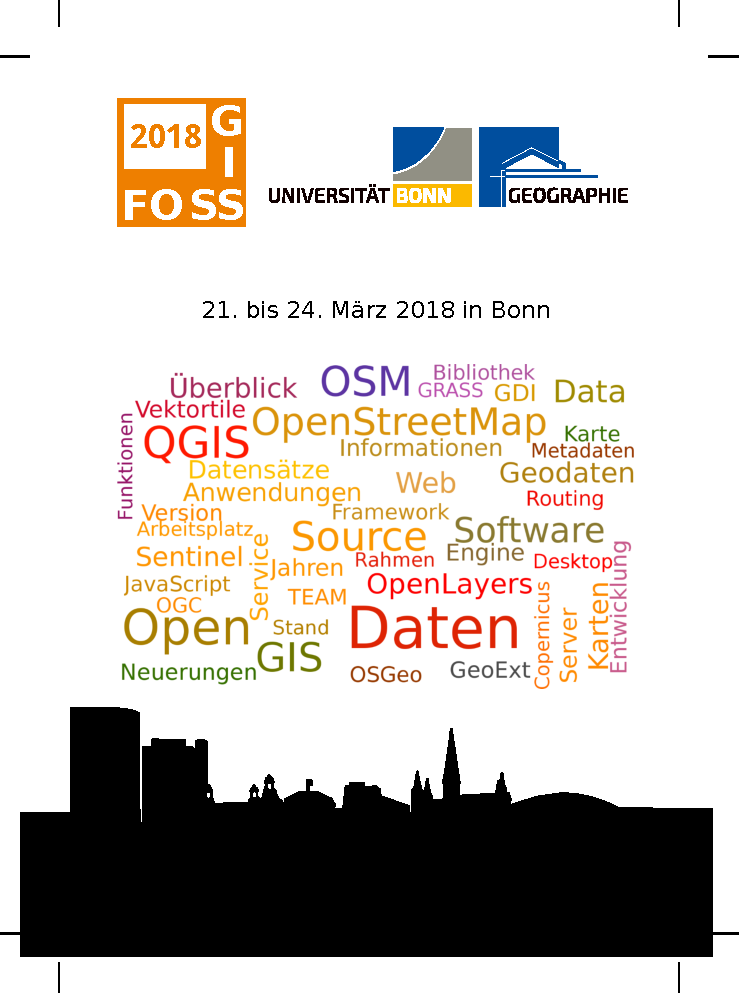
\includegraphics{wallpaper/deckseite-vektor-mit-schnittmarken.pdf}%
}]{titlelayer}
\newpairofpagestyles[]{titlestyle}{}
\AddLayersAtBeginOfPageStyle{titlestyle}{titlelayer}

% define alias commands for all three days
\def\mittwoch{Mittwoch}
\def\donnerstag{Donnerstag}
\def\freitag{Freitag}

% define Wednesday page style
\DeclareNewLayer[background, oddpage,  width=125mm,%
height=169mm, contents={%
  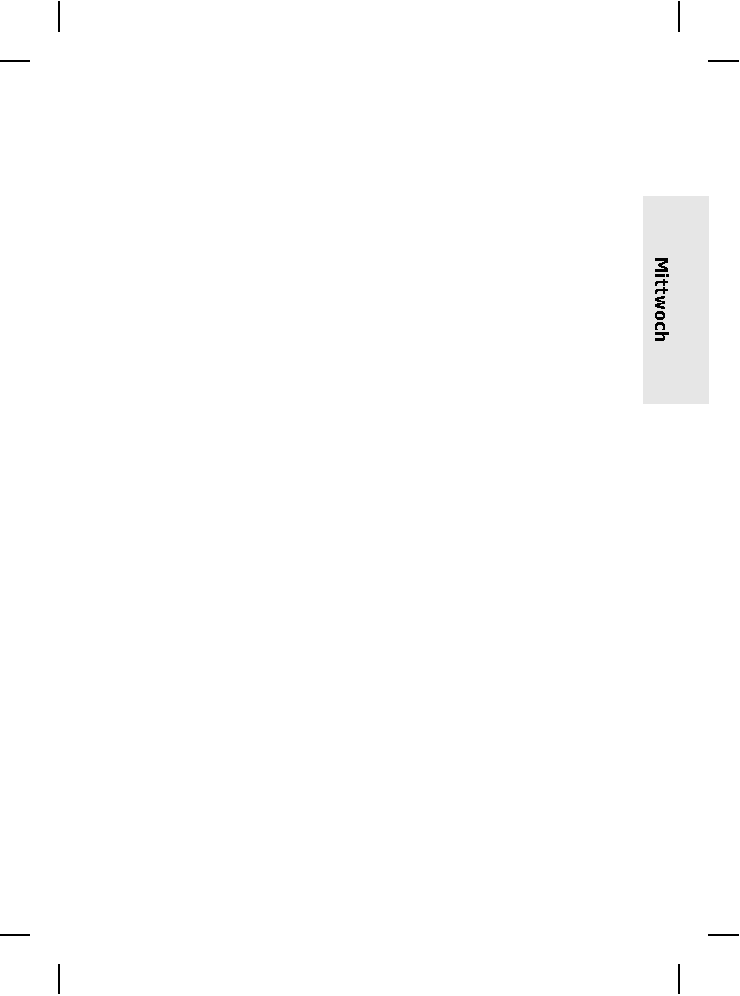
\includegraphics{wallpaper/mittwoch-ungerade.pdf}%
}]{mittwochungerade}
\DeclareNewLayer[background, evenpage,  width=125mm,%
height=169mm, contents={%
  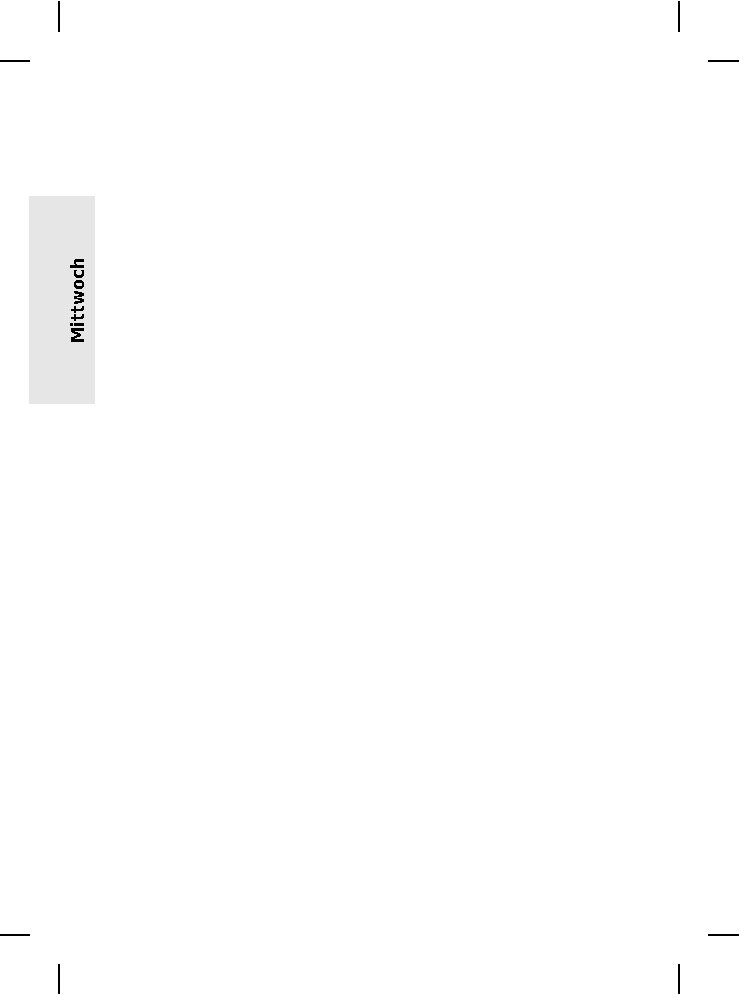
\includegraphics{wallpaper/mittwoch-gerade.pdf}%
}]{mittwochgerade}
\newpairofpagestyles[scrheadings]{mittwoch}{}
\AddLayersAtBeginOfPageStyle{mittwoch}{mittwochgerade}
\AddLayersAtBeginOfPageStyle{mittwoch}{mittwochungerade}

% define Thursday page style
\DeclareNewLayer[background, oddpage,  width=125mm,%
height=169mm, contents={%
  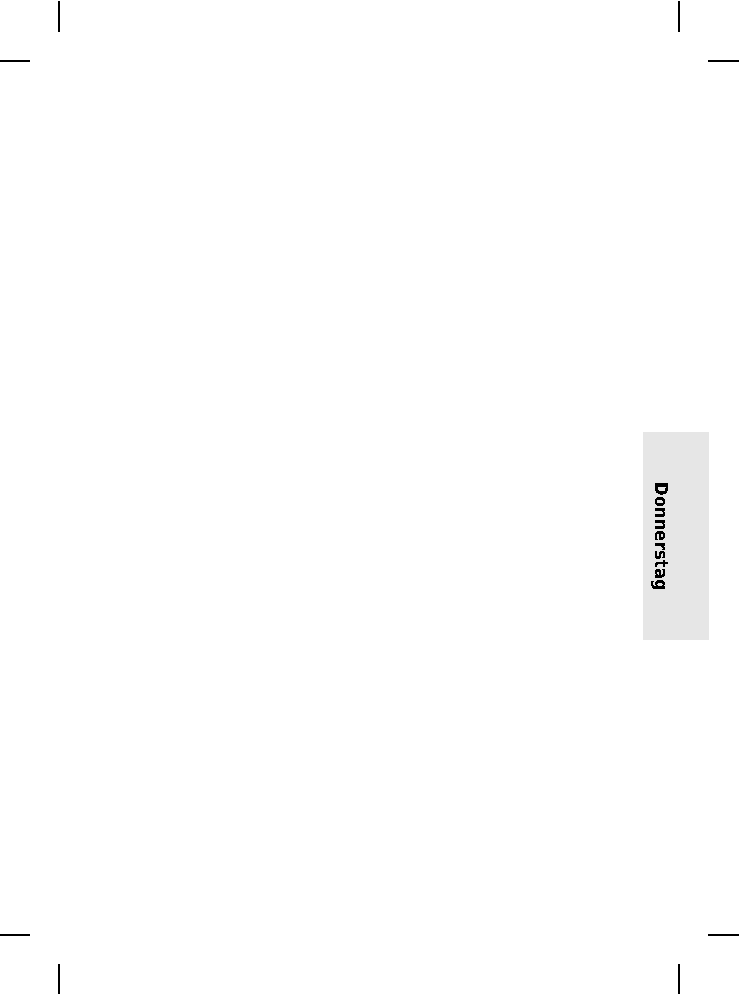
\includegraphics{wallpaper/donnerstag-ungerade.pdf}%
}]{donnerstagungerade}
\DeclareNewLayer[background, evenpage,  width=125mm,%
height=169mm, contents={%
  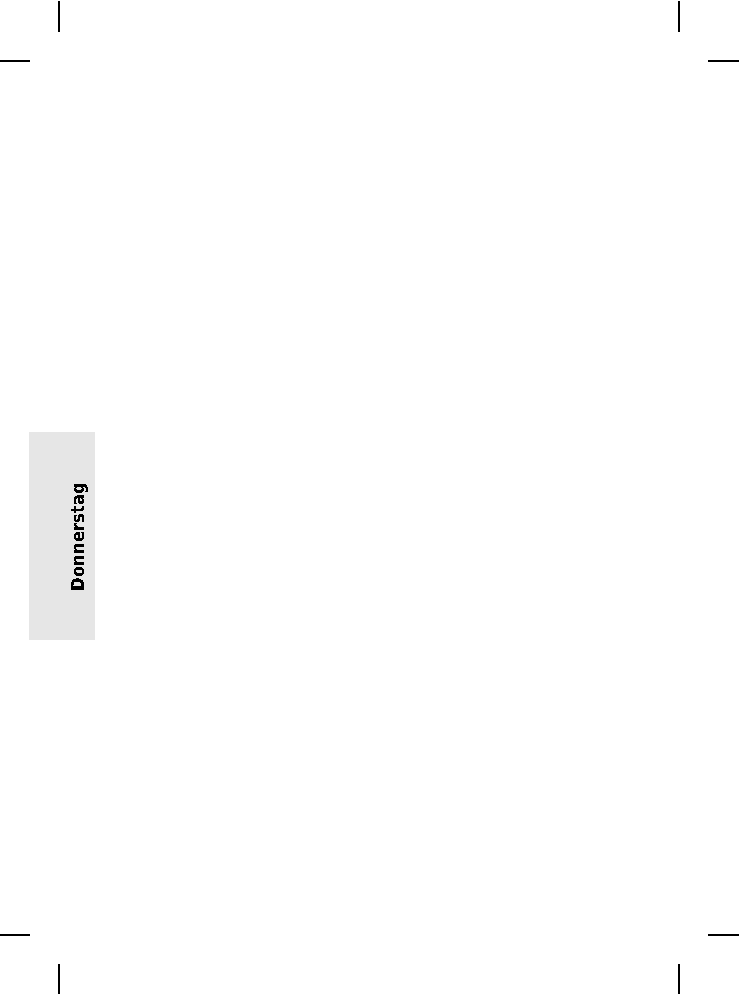
\includegraphics{wallpaper/donnerstag-gerade.pdf}%
}]{donnerstaggerade}
\DeclareNewLayer[background, oddpage,  width=125mm,%
height=169mm, contents={%
  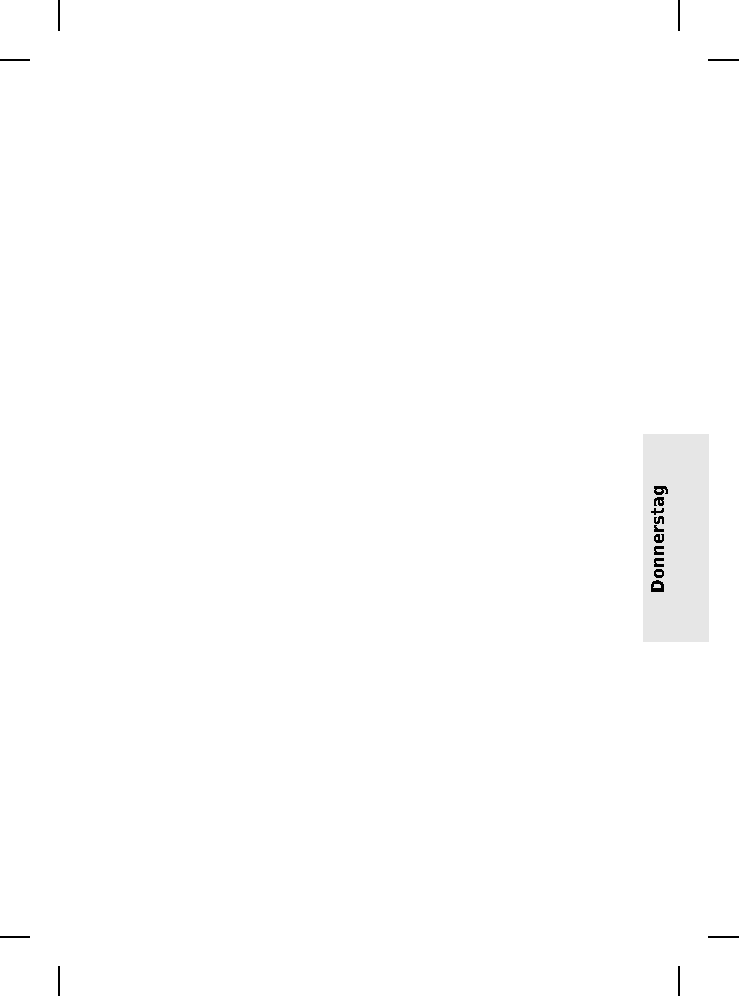
\includegraphics{wallpaper/donnerstag-ungerade-gedreht.pdf}%
}]{donnerstagungeradegedreht}
\newpairofpagestyles[scrheadings]{donnerstag-tabelle}{}
\AddLayersAtBeginOfPageStyle{donnerstag-tabelle}{donnerstaggerade}
\AddLayersAtBeginOfPageStyle{donnerstag-tabelle}{donnerstagungeradegedreht}
\newpairofpagestyles[scrheadings]{donnerstag}{}
\AddLayersAtBeginOfPageStyle{donnerstag}{donnerstaggerade}
\AddLayersAtBeginOfPageStyle{donnerstag}{donnerstagungerade}

% define Friday page style
\DeclareNewLayer[background, oddpage,  width=125mm,%
height=169mm, contents={%
  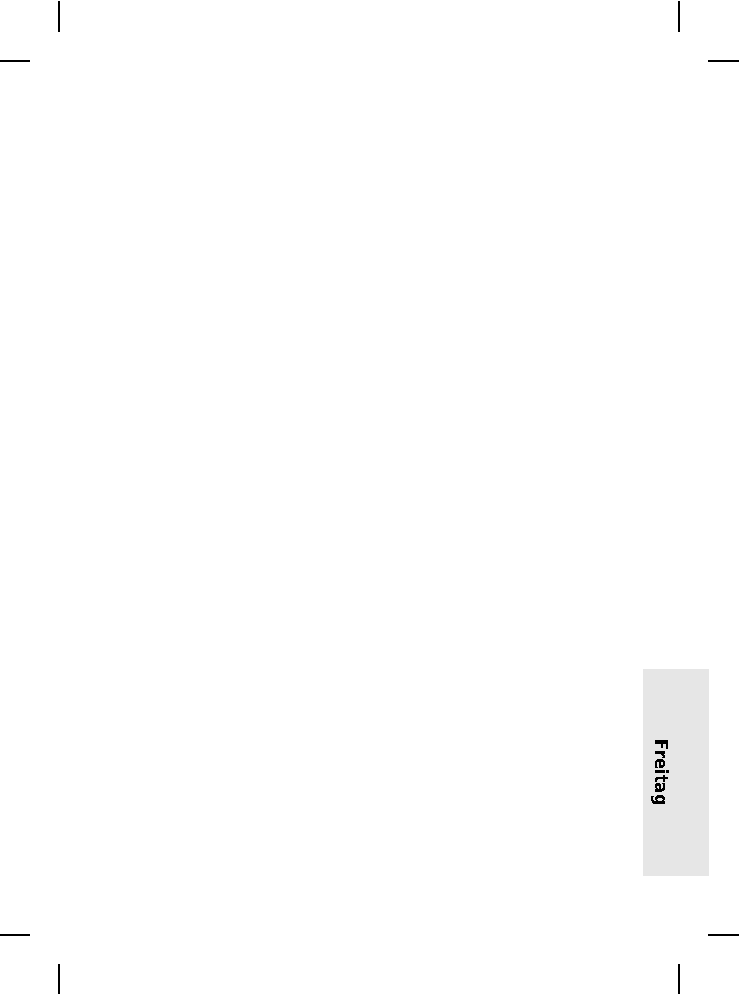
\includegraphics{wallpaper/freitag-ungerade.pdf}%
}]{freitagungerade}
\DeclareNewLayer[background, evenpage,  width=125mm,%
height=169mm, contents={%
  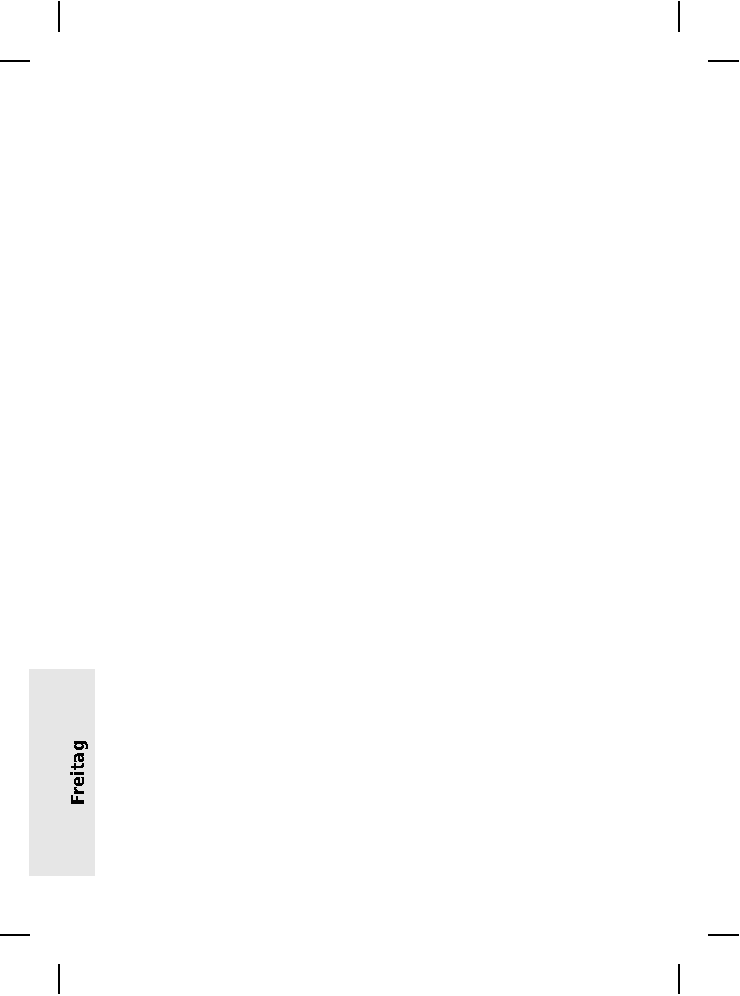
\includegraphics{wallpaper/freitag-gerade.pdf}%
}]{freitaggerade}
\newpairofpagestyles[scrheadings]{freitag}{}
\AddLayersAtBeginOfPageStyle{freitag}{freitaggerade}
\AddLayersAtBeginOfPageStyle{freitag}{freitagungerade}

% \setpagebackground selects the page style to be used depending on the current day. Each day has
% its own page style.
\newcommand{\setpagebackground}{ %
  \ifthenelse{\equal{\conferenceDay}{\mittwoch}}{%
    \pagestyle{mittwoch}
  }{}
  \ifthenelse{\equal{\conferenceDay}{\donnerstag}}{%
    \pagestyle{donnerstag}
  }{}
  \ifthenelse{\equal{\conferenceDay}{\freitag}}{%
    \pagestyle{freitag}
  }{}
}


% additional column type for tables
\newcolumntype{Y}[1]{>{\RaggedRight\arraybackslash}p{#1}}

%% length of the title boxes
\newlength{\titleboxwidth}
\setlength{\titleboxwidth}{\textwidth}
\advance\titleboxwidth by -6pt

% command to lay out the title boxes
\newcommand{\setabstract}[6]{
	% 1. speaker
	% 2. title
	% 3. subtitle
	% 4. abstract (Text)
	% 5. colour
	% 6. room
	%\thispagestyle{scrheadings}
  \setpagebackground
	\setlength\tabcolsep{0pt}
	% \setlength{\fboxsep}{0pt}
	\noindent\fcolorbox{white}{#5}{\parbox{\titleboxwidth}{%
		\noindent\begin{tabu}{X[5L]r}
			\isspeakerempty{#1}{#2}{#6}
			\issubtitleempty{#3}
		\end{tabu}%
	}}
	%
	\isabstractempty{#4}%
	\vspace{0.5em}% space to the next talk even if there is no abstract
	\setlength\tabcolsep{6pt} % set column padding back to default value
}

% lay out the speaker if there is any
% We assume that there is only a subtitle if the talk has a speaker.
\makeatletter
\newcommand{\isspeakerempty}[3]{%
	% Arguments:
	% 1. speaker
	% 2. title
	% 3. room
	\@ifmtarg{#1}{%
			\par\noindent\large \sectfont #2% % titel
			&
			#3, \talktime
			\tabularnewline
		}
		{
			\emph{#1} % Sprecher
			&
			\talktime
			\tabularnewline
			{\par\noindent\large \sectfont #2}% % titel
			&
			#3
			\tabularnewline
		}
		
}
\makeatother

% Lay out the subtitle
% has to be a separate function and has to be surrounded by \makeatletter for technical reasons
\makeatletter
\newcommand{\issubtitleempty}[1]{%
	\@ifnotmtarg{#1}{\multicolumn{2}{Y{\linewidth}}{\vspace{-0.6em} \noindent\bfseries \normalsize \sectfont #1}\tabularnewline}
}
\makeatother

% Lay out the abstract if there is any
% has to be a separate function and has to be surrounded by \makeatletter for technical reasons
\makeatletter
\newcommand{\isabstractempty}[1]{%
		\vspace{0.5em}\newline%
		#1 \par% % abstract
		\vspace{1.5em}% space to the next talk even if there is an abstract
}
\makeatother

% define colours
%\definecolor{eins}{cmyk}{ 0 .18 .06 .10}
\definecolor{eins}{cmyk}{ 0 .13 .04 .08}
\definecolor{zwei}{cmyk}{ .1 0 .17 .05}
\definecolor{hellorange}{cmyk}{ 0 0.18 0.40 0.03}
%\definecolor{aula}{cmyk}{ 0.2 0 0.05 0.13}
\definecolor{aula}{cmyk}{ 0.13 0 0.04 0.11}
\definecolor{geoblau}{cmyk}{ 0.24 .02 0 .01}
\definecolor{dezentrot}{cmyk}{ 0 .24 0.29 .04}
\definecolor{hellgelb}{cmyk}{ 0 .02 0.36 0}
\definecolor{hellgruen}{cmyk}{ 0.10 .0 0.22 0.05}

% abstract at Wolfgang-Paul-Hörsaal
\newcommand{\abstractWPH}[4]%
{%
	\setabstract{#1}{#2}{#3}{#4}{aula}{WPH}
}

% abstract at Alfred-Philippson-Hörsaal
\newcommand{\abstractAPH}[4]%
{%
	\setabstract{#1}{#2}{#3}{#4}{hellgelb}{APH}
}

% abstract at Hörsaal 2
\newcommand{\abstractZwei}[4]%
{%
	\setabstract{#1}{#2}{#3}{#4}{hellgruen}{HS 2 GZ}
}

% abstract at Hörsaal 4
\newcommand{\abstractVier}[4]%
{%
	\setabstract{#1}{#2}{#3}{#4}{geoblau}{HS 4 GZ}
}

% abstract at a different location
\newcommand{\abstractOther}[5]%
{%
	\setabstract{#1}{#2}{#3}{#4}{hellorange}{#5}
}

% infobox for workshops (they don't have an abstract in the booklet)
\newcommand{\workshopbox}[3]%
{%
	% 1. titel
	% 2. speaker
	% 3. Room
	\setlength\tabcolsep{0pt}
	\noindent\fcolorbox{white}{dezentrot}{\parbox{\titleboxwidth}{%
			\noindent
			\begin{tabu}{X[5L]r}
				\emph{#2} % Sprecher
				&
				\talktime
				\tabularnewline
				{\noindent\large \bfseries #1}% % title
				&
				#3
				\tabularnewline
			\end{tabu}
		}
	}
	\setlength\tabcolsep{6pt} % set column padding back to default
}

% too long
\newcommand{\tooLong}{Dieser Text ist viel zu lang. Dieser Text ist viel zu lang. Dieser Text ist viel zu lang. Dieser Text ist viel zu lang. Dieser Text ist viel zu lang. Dieser Text ist viel zu lang. Dieser Text ist viel zu lang. Dieser Text ist viel zu lang. Dieser Text ist viel zu lang. Dieser Text ist viel zu lang. Dieser Text ist viel zu lang. Dieser Text ist viel zu lang. Dieser Text ist viel zu lang. Dieser Text ist viel zu lang. }

\newlength{\fboxwidth}

\def\workshopsSection{workshopsSection}
\def\abstractsSection{abstractsSection}

% boxes for advertisement texts by our sponsors
\newcommand{\sponsorenbox}[4]{%
  \setlength{\fboxwidth}{\textwidth}
  \advance\fboxwidth by -7.0pt
  \abstractSponsorenbox{#1}{#2}{#3}{#4}{\workshopsSection}%
}

\newcommand{\sponsorenboxA}[4]{%
  \setlength{\fboxwidth}{\textwidth}
  \advance\fboxwidth by -10.0pt
  \abstractSponsorenbox{#1}{#2}{#3}{#4}{\abstractsSection}%
}

%% Sponsorenbox
%% 1. Logo
%% 2. Logobreite
%% 3. Anzahl benötigter Zeilen
%% 4. Text
%% 5. Umfeld (\workshopsSection oder \abstractsSection}
\makeatletter
\newcommand{\abstractSponsorenbox}[5]{%
  \setlength{\fboxsep}{4.5pt}%
  \noindent%
  \ifthenelse{\equal{#5}{\workshopsSection}}{%
    \hspace{2.65pt}%
  }{\hspace{-1pt}}%
  \fcolorbox{gray}{white}{\parbox{\fboxwidth}{
    \@ifmtarg{#1}{}{%
      \begin{wrapfigure}[#3]{r}[0pt]{#2}
        \centering\vspace{-1\baselineskip}
        \includegraphics[width=#2]{#1}
      \end{wrapfigure}
    }

    \noindent #4
  }}
  \setlength{\fboxsep}{3pt}
}
\makeatother

% Definitionen für Tagestabellen
\newcolumntype{Z}[1]{>{\RaggedRight\arraybackslash}p{#1}}%
\newcolumntype{C}[1]{>{\Centering\arraybackslash}p{#1}}%
\newcommand{\talk}[2]%
{%
	& \textbf{#1}
        \ifthenelse{\equal{#2}{}}%
        {}%
        {\newline\emph{#2}}
}%
% Titel -- Redner


\newcommand{\workshop}[3]%
{%
	\workshopbox{#1}{#2}{#3}
}%

\newcommand{\otherevent}[1]%
{%
	& \textbf{#1}
}%

\newcommand{\aulaevent}[2]%
{%
	&
	\multicolumn{3}{c}{
		\textbf{#1} (Aula) \par \emph{#2}
	}
}%

\newcommand{\coffeespace}{\vspace{0.4em}}
\newcommand{\workshopspace}{\vspace{0.5em}\\}

% Farben definieren
\definecolor{commongray}{gray}{.9}
%\vspace{-1.2em}
\renewcommand{\arraystretch}{1.4}



\begin{document}
\lsstyle
\usefont{T1}{DejaVuSansCondensed-TLF}{m}{n}
 
\pagestyle{cropmarksstyle}
\begin{titlepage}
  \thispagestyle{titlestyle}
  \null
\end{titlepage}
\pagestyle{cropmarksstyle}

\selectlanguage{ngerman}
\section*{Inhalt}

\vspace*{0.35em}%
\noindent Workshops am Mittwoch \dotfill \pageref{mittwoch-workshops}

\vspace*{0.35em}%
\noindent Workshops am Donnerstag \dotfill \pageref{donnerstag-workshops}

\vspace*{0.35em}%
\noindent Workshops am Freitag \dotfill \pageref{freitag-workshops}

\vspace*{0.35em}%
\noindent Vorträge am Mittwoch \dotfill \pageref{mittwoch}

\vspace*{0.35em}%
\noindent Vorträge am Donnerstag \dotfill \pageref{donnerstag}

\vspace*{0.35em}%
\noindent Vorträge am Freitag \dotfill \pageref{freitag}

\vspace*{0.35em}%
\noindent OSM-Samstag \dotfill \pageref{osm-samstag}

\vspace*{0.35em}%
\noindent Raumplan \dotfill \pageref{raumplan-page}

\vspace*{0.35em}%
\noindent Impressum \dotfill \pageref{impressum}
\newpage

\newpage
\section*{Willkommen zur FOSSGIS-Konferenz 2018 in Bonn!} \label{welcome}
Die Abkürzung FOSSGIS steht
%\emph{FOSSGIS} ist eine Abkürzung
für freie und Open"=Source"=Software für Geoinformationssysteme.
Die FOSSGIS"=Konferenz ist im deutschsprachigen Raum die führende Konferenz zu diesem Thema
und wird dieses Jahr vom gemeinnützigen FOSSGIS e.V und der OpenStreetMap"=Community
gemeinsam mit der Rheinischen Friedrich-Wilhelms-Universität Bonn organisiert.

Ziel der jährlich stattfindenden Konferenz ist die Verbreitung von freier und
Open-Source-Software für Geoinformationssysteme.  In den nächsten vier Tagen
haben Sie die Gelegenheit, sich mit Anwendern und Entwicklern auszutauschen und
neuste Informationen zu Anwendungs- und Arbeitsmöglichkeiten zu erhalten. Im
Foyer des Geozentrums werden Firmen und Projekte ihr Knowhow präsentieren.

Die FOSSGIS-Konferenz findet in den Gebäuden der Geographie, der Kartographie und dem Geozentrum auf dem Campus Poppelsdorf statt.

\newpage
% \section*{Goldsponsor}
\begin{center}
	
\includegraphics[width=0.6\textwidth]{001_Wheregroup}
\end{center}
Die WhereGroup gehört in Detuschland zu den führenden Anbietern von Geoinformationssystemen mit
Open-Source-Software. Wir bieten alle Dienstleistungen rund um Beratung, Konzeption, Entwicklung,
Aufbau und Betrieb dynamischer Kartenanwendungen im Intra- und Internet. Darüber hinaus gehört ein
umfangreiches Schu\-lungs- und Workshop-Programm zu unserem Portfolio.

Gegründet wurde das Unternehmen als eine Fusion drei verschiedener Unternehmen in Bonn. Im Jahr 2017
haben wir unser 10-jähriges Jubiläum gefeiert. Das WhereGroup"=Team umfasst heute über 30 Angestellte
unterschiedlicher Fachrichtungen -- verteilt auf die Standorte Bonn (Hauptsitz), Freiburg und Berlin.

Das Spektrum unserer Lösungen reicht von Geoportalen und kartenbasierter
Datenverwaltung bis hin zu hochverfügbaren Anwendungen für die freie Wirtschaft und die öffentliche
Verwaltung.

In unseren Projekten setzen wir auf die Standards bzw. Empfehlungen des Open Geospatial
Consortiums (OGC), der INSPIRE"=Richtlinie sowie der GDI"=DE. Ihre Verwendung gewährleistet ein Maximum
an Interoperabilität und Flexibilität unserer Lösungen. Die Einhaltung hoher Sicherheitsstandards
ist für uns nicht zuletzt durch unsere Projekte mit Landes- und Bundesbehörden sowie Großkonzernen
eine Selbst\-ver\-ständ\-lichkeit.

Wir beraten absolut herstellerunabhängig und sind spezialisiert auf die Weiterentwicklung,
professionelle Anwendung und Integration offener Standards und bewährter
Open"=Source"=Technologien und freier Software. Dazu zählen neben unseren Projekten Mapbender\,3,
MetaDor\,2 und PostNAS u.\,a. GeoServer, MapServer, MapProxy, OpenLay\-ers, PostGIS, QGIS und
OpenStreetMap.

Über unser Schulungsinstitut, die FOSS Academy, bieten wir praxisorientierte
Schulungen zum Thema "`GIS mit Open-Source-Software"' an. Diese können sowohl von Einzelpersonen als
auch von Firmen, auf Wunsch auch als Inhouse-Schulungen, gebucht werden.
Zu unserer Überzeugung
gehört, dass wir uns aktiv in die Geoinformatik-Community einbringen. Es ist uns wichtig, an der
Diskussion und Weiterentwicklung von verschiedensten Open-Source-Lösungen mitzuwirken.

\enlargethispage{1.5\baselineskip}
Die WhereGroup ist bundesweit und international mit Hochschulen, Firmen und Verbänden vernetzt. Wir
verfügen über langjährige, persönliche Kontakte zu diversen Universitäten und Hochschulen im In- und
Ausland, zum FOSSGIS e.V., zur Open Source Geospatial Foundation (OSGeo), zum Open Geospatial
Consortium (OGC), sowie zu den Herstellern bzw. Maintainern der gängigsten Open-Source-Produkte im
Geo-Bereich.  Mehr zur WhereGroup unter www.wheregroup.com und www.foss-academy.com.


\section*{Workshops am Mittwoch}\label{mittwoch-workshops}%
\newsmalltimeslot{10:30 bis 12:00}%
% Hack, um Einrücken des ersten Workshops wieder rückgängig zu machen
\RaggedRight
\noindent\workshop{react-geo -- Mapping mit React}{André Henn}%
{Übungsraum~1}\workshopspace
\noindent\workshop{Entwicklung von QGIS-Plugins mit Python}{Sören Gebbert, Marco Hugentobler}%
{Übungsraum~6}\workshopspace
\noindent\workshop{GeoServer-Vertiefung}{Nils Bühner}%
{Gislabor}\workshopspace
\newsmalltimeslot{15:00 bis 16:30}
\noindent\workshop{Geodatenverarbeitung mit \mbox{SpatialSQL}}{Claas Leiner}%
{Übungsraum~1}\workshopspace
\noindent\workshop{QGIS 3}{Klaus Mithöfer, Otto Dassau}%
{Übungsraum~6}\workshopspace
\noindent\workshop{Erste Schritte mit geometrischen Objekten in Python}{Johannes Kröger}%
{Gislabor}\workshopspace

\newpage
\section*{Workshops am Donnerstag}\label{donnerstag-workshops}
\newsmalltimeslot{09:00 bis 10:30}
\noindent\workshop{Vektortiles erstellen und publizieren}{Pirmin Kalberer}%
{Übungsraum~1}\workshopspace
\noindent\workshop{Webmapping-Basics mit Leaflet}{Numa Gremling}%
{Übungsraum~6}\workshopspace
\noindent\workshop{QGIS-Modeller-Einstieg}{Claas Leiner}%
{Gislabor}\workshopspace
\newsmalltimeslot{11:05 bis 12:35}
\noindent\workshop{Einführung in den MapServer}{Jörg Thomsen}%
{Übungsraum~1}\workshopspace
\enlargethispage{1\baselineskip}
\noindent\workshop{Prozessierung von Copernicus Daten mit freier (Kommandozeilen-)Software}{Carmen Tawalika}%
{Übungsraum~6}\workshopspace
\noindent\workshop{Fusion von Geo- und Statistikdaten mit R}{Benedikt Gräler}%
{Gislabor}\workshopspace
\newpage
\newsmalltimeslot{13:40 bis 15:10}
\vspace*{1.15\baselineskip}
\noindent\workshop{GitLab}{Arne Schubert, Stephan Herritsch}%
{Übungsraum~1}\workshopspace
\noindent\workshop{Finden und Korrigieren von Geometrie- und Topologiefehlern}{Klaus Mithöfer, Otto Dassau}%
{Übungsraum~6}\workshopspace
\noindent\workshop{Einführung in GeoServer}{Daniel Koch}%
{Gislabor}\workshopspace
\noindent\workshop{Open Database License}{Falk Zscheile}%
{Roter Saal}\workshopspace
\newsmalltimeslot{15:45 bis 17:15}
\noindent\workshop{INSPIRE-Downloadservice mit Deegree und PostgreSQL}{Torsten Friebe}%
{Übungsraum~6}\workshopspace
\noindent\workshop{Einführung in PostGIS}{Jörg Thomsen}%
{Gislabor}\workshopspace
% reduce \arraystretch to make all boxes fit on a single page
\renewcommand{\arraystretch}{1.3}
\renewcommand{\arraystretch}{1.4}

\newpage
\section*{Workshops am Freitag}\label{freitag-workshops}
\enlargethispage{1\baselineskip}
\newsmalltimeslot{09:00 bis 10:30}
\noindent\workshop{PostgreSQL/PostGIS für Fortgeschrittene}{Astrid Emde}%
{Übungsraum~1}\workshopspace
\noindent\workshop{Geodaten jonglieren mit ogr2ogr}{Claas Leiner}%
{Übungsraum~6}\workshopspace
\noindent\workshop{QGIS-Symbole mit Inkscape individuell erstellen}{Katrin Hannemann}%
{Gislabor}\workshopspace
\newsmalltimeslot{11:05 bis 12:35}
\noindent\workshop{Karten aus QGIS ins Buch, Web oder auf die Leinwand}{Johannes Kröger}%
{Übungsraum~1}\workshopspace
\noindent\workshop{Geodatenverarbeitung mit GRASS GIS}{Markus Neteler}%
{Übungsraum~6}\workshopspace
\noindent\workshop{Micro-Service Geo-Daten-Infrastrukturen mit Docker}{Arne Schubert}%
{Gislabor}\workshopspace

\newpage
\renewcommand{\arraystretch}{1.4}
\section*{Vorträge am Mittwoch}\label{mittwoch}
\renewcommand{\conferenceDay}{\mittwoch}
\setpagebackground
\noindent\begin{tabular}{Z{0.85cm}Z{6.85cm}}
  & \multicolumn{1}{c}{\cellcolor{hellgruen} Hörsaal 2 (Geozentrum)}
  \tabularnewline
  10:30
  \talk{Die Open-Source-Software}{}
  \tabularnewline
  \rowcolor{commongray}
  12:00 & \multicolumn{1}{c}{%
    \parbox[c]{24pt}{%
      
\includegraphics[height=10pt]{cafe}%
    }
    Pause
  } \tabularnewline
\end{tabular}

\vspace{1.5\baselineskip}
\noindent\begin{tabular}{Z{0.85cm}Z{6.85cm}}
  & \multicolumn{1}{c}{\cellcolor{aula} Wolfgang-Paul-Hörsaal} \tabularnewline
  13:00
  \talk{Eröffnungs\-veranstaltung}{}
  \tabularnewline
  13:25
  \talk{Erfahrungen u. Aussichten bei OpenNRW}{Andre Caffier}
  \tabularnewline
  13:50
  \talk{OSGeo, Location Tech und Open Source als Geschäftsmodell}{Marc Vloemans}
  \tabularnewline
  14:15
  \talk{Lightning Talks}{}
  \tabularnewline
  \rowcolor{commongray}
  14:30 & \multicolumn{1}{c}{%
    \parbox[c]{24pt}{%
      
\includegraphics[height=10pt]{cafe}%
    }
    Kaffeepause} \tabularnewline
\end{tabular}

\vspace{1.5\baselineskip}
\enlargethispage{1.0\baselineskip}
\renewcommand{\arraystretch}{1.3}
\noindent\begin{tabular}{lZ{2.0cm}Z{2.0cm}Z{2.0cm}}
  & \multicolumn{1}{c}{\cellcolor{hellgelb} APH}
  & \multicolumn{1}{c}{\cellcolor{hellgruen} HS\,2}
  & \multicolumn{1}{c}{\cellcolor{geoblau} HS\,4}
  \tabularnewline
  15:00
  \talk{GRASS GIS 7.4.0}{Markus Neteler}
  \talk{XPlanung 5.0 in QGIS}{Bernhard Ströbl}
  \talk{Wir reden doch alle vom Standard?}{Till Adams}
  \tabularnewline
\end{tabular}
\newpage
  
\begin{center}
  \renewcommand{\arraystretch}{1.3}
  \noindent\begin{tabular}{lZ{2.0cm}Z{2.0cm}Z{2.0cm}}
    & \multicolumn{1}{c}{\cellcolor{hellgelb} APH}
    & \multicolumn{1}{c}{\cellcolor{hellgruen} HS\,2}
    & \multicolumn{1}{c}{\cellcolor{geoblau} HS\,4}
    \tabularnewline
    15:35
    \talk{OpenLayers}{Marc Jansen}
    \talk{XPlanung u. \mbox{INSPIRE} PLU}{Dirk Stegner}
    \talk{WMS Time Dimension}{Armin Retterath}
    \tabularnewline
    16:10
    \talk{QGIS Web Client 2}{Pirmin Kalberer}
    \talk{Radrouten\-speicher Metropole Ruhr}{David Arndt}
    \talk{GeoHealth\-Check}{Just van der Broecke}
    \tabularnewline
    \rowcolor{commongray}
    16:35 & \multicolumn{3}{c}{%
    \parbox[c]{24pt}{%
      
\includegraphics[height=10pt]{cafe}%
    }
    Kaffeepause} \tabularnewline
    17:05
    \talk{Neues von GeoServer}{Nils Bühner}
    \talk{pyramid\newline\_oereb}{Clemens Rudert}
    \talk{Offene Geodaten aus NRW}{Markus Neteler}
    \tabularnewline
    17:40
    \talk{Idproxy}{Sven Böhme}
    \talk{ALKIS kompakt mit SpatiaLite}{Claas Leiner}
    \talk{OpenMeta\-Data}{Sebastian Goerke}
    \tabularnewline
    18:10
    \talk{Mapbender}{Axel Schäfer}
    \talk{geOrchestra}{Emmanuel Belo}
    \talk{OpenDEM Europe}{Martin Over}
    \tabularnewline
    \rowcolor{commongray}
    18:30 &
    \multicolumn{3}{c}{%
      Anwendertreffen (siehe Seite \pageref{bof-mittwoch})}
    \tabularnewline
    \rowcolor{commongray}
    19:15 &
    \multicolumn{3}{c}{%
      \parbox[c]{24pt}{%
        
\includegraphics[height=10pt]{restaurant}%
      }
      Campus-Dialoge in der Mensa Poppelsdorf}
    \tabularnewline
  \end{tabular}
\end{center}
\renewcommand{\arraystretch}{1.0}

\newpage



% 10:30
\renewcommand{\conferenceDay}{\mittwoch}
\newsmalltimeslot{10:30}
\abstractZwei{Dominik Helle, Astrid Emde, Till Adams, Marco Lechner}%
{Was sind "`Open"' Source, Data und Standards - und wie funktioniert das?}%
{}%
{Open Source hat viele Facetten -- und es ranken sich inzwischen ebenso viele Mythen darum. Was
davon richtig ist und was nicht, stellen wir in einer kurzen Einführung zusammen. Was sind Open Data
und Open Standards, welche Gemeinsamkeiten gibt es und wo unterscheiden sie sich? Der Vortrag
richtet sich an alle, die mit Open Source, Open Data oder Open Standards bisher noch wenig Kontakt
hatten und die Grundlagen verstehen möchten.}

% 13:00
\newsmalltimeslot{13:00}%
\abstractWPH{Marco Lechner}%
{Eröffnungsveranstaltung der FOSSGIS-Konferenz 2018}%
{}%
{Begrüßung durch den Veranstalter der Konferenz (FOSSGIS e.V.) und Grußworte der gastgebenden Universität}
\enlargethispage{1\baselineskip}

\newsmalltimeslot{13:25}%
\abstractWPH{Andre Caffier}%
{Erfahrungen und Aussichten bei OpenNRW}%
{}%
{}

\newsmalltimeslot{13:50}
\abstractWPH{Marc Vloemans}%
{OSGeo, LocationTech und Open Source als Geschäftsmodell}%
{}{}

\newsmalltimeslot{14:15}%
\abstractWPH{}%
{Lightning Talks}%
{}%
{%
  \vspace{-2em}
  \begin{itemize}
    \RaggedRight
    \setlength{\itemsep}{-2pt} % Aufzählungspunktabstand auf 0
    \item \emph{Jörg Thomsen:} Private Open Data
    \item \emph{Jakob Miksch:} Geodaten mit LightOnEurope intuitiv erkunden
    \item \emph{Till Adams:} Think Big -- der FOSSGIS e.V. als Großkonzern
  \end{itemize}
  \justifying
}

% 15:00
\newtimeslot{15:00}
\abstractAPH{Markus Neteler}%
{Neues aus dem GRASS GIS Projekt: die 7.4.0 Version steht bereit}%
{}%
{
Auch nach über 30 Jahren seit der ersten Version kann GRASS GIS mit modernen Features aufwarten.
Nach fast einjähriger Entwicklungszeit steht die neue stabile GRASS GIS 7.4 zur Verfügung. Das
Entwicklerteam hat die Benutzerfreundlichkeit weiter verbessert, Addons in das Kernpaket migriert
und die Orthorektifikation von Luftbildern überarbeitet. Die Rasterdatenspeicherung wurde auch im
Hinblick auf die Cloud-Verarbeitung von massiven Datensätzen weiter optimiert und neue
Vektoralgorithmen integriert. Alles steht auch auf dem Docker Hub zur Verfügung.
}


\abstractZwei{Bernhard Ströbl}%
{XPlanung 5.0 in QGIS}%
{}%
{
Die Stadtverwaltung Jena benutzt seit ca. zwei Jahren XPlanung in Verbindung mit QGIS. Sowohl die
Datenmodellierung in PostGIS als auch die Benutzeroberfläche für QGIS wurden komplett im eigenen
Haus entwickelt und stehen als freie Software zur Verfügung. Seit Ende 2017 ist der neue Standard
XPlanung 5.0 implementiert. Der Vortrag beschreibt die Entwicklung der Datenmodellierung und der
Software sowie ihre Anwendung in der Praxis. Sowohl Entwickler als auch Anwender stehen gern zum
Gespräch und Erfahrungsaustausch zur Verfügung.
}


\abstractVier{Till Adams}%
{Wir reden doch alle Standard -- oder etwa nicht?}%
{Was tun mit WMS, WFS und WCS, SHP, XML und MXD -- MFG?}%
{
GDAL, OGR, PDAL, GEOS und FDO -- und am Ende brauchen doch alle FME?
Die Open Source GIS-Welt bietet eine Vielzahl an Lösungen, davon sind viele lebendig, andere
geistern als nicht mehr gepflegte Werkzeuge immer noch im WWW herum.  Der Vortrag stellt Lösungen
für Datenkonvertierung und Systemmigration anhand von anschaulichen Beispielen vor dem Schwerpunkt
der Migration von GI-Werkzeugen vor. Und warnt vor denen, die es eigentlich nicht mehr gibt.%
}

\newtimeslot{15:35}
% time: 2018-03-21 15:35:00
\abstractAPH{Marc Jansen}%
{OpenLayers}%
{Stand und Zukunft}%
{
OpenLayers ist eine sehr bekannte und verbreitete Open-Source-JavaScript-Bibliothek, um interaktive
Karten im Web aus verschiedenste Quellen mit reichhaltigen Interaktionsmöglichkeiten zu erstellen.
Seit mehr als zehn Jahren wird OpenLayers stets weiterentwickelt und ist auch im Jahre 2018 eine
moderne Bibliothek, die ihren Benutzern eine Fülle an Optionen an die Hand gibt, um auch
anspruchsvollste webbasierte Kartenapplikation zu erstellen.

Im Vortrag von OpenLayers Kernentwicklern werden aktueller Stand und zukünftige Entwicklungen
beleuchtet.%
}

% time: 2018-03-21 15:35:00
\abstractZwei{Dirk Stenger}%
{Datenaustausch in der Bauleitplanung effizienter gestalten mit XPlanung und INSPIRE PLU}%
{}%
{
Der Vortrag stellt eine auf Open-Source-Software basierte Lösung vor, um den Datenaustausch in der
Planung effizienter zu gestalten, und zeigt die Abbildung von Prozessen zur Verwaltung der Planwerke
innerhalb einer PostGIS-Datenhaltung sowie Validierung von XPlanGML-Dateien. Zudem wird die
Publikation der Daten über deegree Dienste vorgestellt.  Einen Schwerpunkt nimmt die Fragestellung
ein, wie im XPlanGML-Format vorliegende Daten in das INSPIRE Planned Land Use (PLU) Schema überführt
und über INSPIRE-konforme Netzwerkdienste publiziert werden können.%
}

% time: 2018-03-21 15:35:00
\abstractVier{Armin Retterath}%
{WMS Time Dimension}%
{Mehrwert für Geodateninfrastrukturen}%
{
Die zunehmende Zahl an Metadaten in Geodateninfrastrukturen macht eine Informationsrecherche immer
schwieriger. Es werden oft Datensätze mehrfach beschrieben, die sich nur hinsichtlich ihrer
zeitlichen Dimension voneinander unterscheiden. Bei der Bereitstellung durch Dienste wirkt sich das
dann so aus, dass es beispielsweise für jedes Jahr einen eigenen Layer gibt. Hier kann eine die
Verwendung von zeitlich variablen WMS-Layern Abhilfe schaffen. Im Vortrag wird der generische Ansatz
der GDI-RP anhand von praktischen Beispielen vorgestellt.%
}

\newtimeslot{16:10}
% time: 2018-03-21 16:10:00
\abstractAPH{Pirmin Kalberer}%
{QGIS Web Client 2}%
{}%
{
QGIS Web Client 2 (QWC2) ist die zweite Generation des QGIS-Webclients, einem Web-GIS-Client
optimiert für QGIS-Server. Er unterstützt die Erweiterungen des QGIS-Servers für PDF-Druck, Suche,
Datenexport, Legenden etc. QWC~2 wurde mit responsivem Design und modular entwickelt. Die identische
Version läuft auf Tablets, Mobiltelefonen und Desktop-Rechnern.

Der Vortrag gibt einen kurzen Überblick über die Funktionalität und zeigt die letzten
Weiterentwicklungen (z.\,B. Digitalisieren). Ebenfalls kurz vorgestellt wird ein exemplarisches
Server-Setup.%
}


% time: 2018-03-21 16:10:00
\abstractZwei{David Arndt}%
{Radroutenspeicher Metropole Ruhr}%
{}%
{
Das Geonetzwerk metropoleRuhr ist seit Januar 2016 aktiv in der Abstimmung zur digitalen
Führung der Radwege. Zur Erleichterung der digitalen Erfassung hat der Regionalverband
Ruhr eine Web-GIS Anwendung "`Mapbender Radroutenspeicher Metropole Ruhr"' sowie ein
QGIS-Projekt erstellt.
Durch die Nutzung der Anwendung und des QGIS-Projektes wird bei der Pflege
des Datenbestandes "`Radrouten"' sichergestellt, dass keine redundante Datenhaltung bei den
Verbandsmitgliedern vorliegt und gemeinsam in einen Primärdatenbestand eingearbeitet wird.%
}

% time: 2018-03-21 16:10:00
\abstractVier{Just van den Broecke}%
{GeoHealthCheck}%
{Uptime and QoS monitor for geospatial web-services}%
{
  \begin{otherlanguage}{english}
    Keeping Geospatial Web Services up-and-running is best accommodated by continuous monitoring.  Not
    only downtime needs to be guarded but also whether the services are functioning correctly and do not
    suffer from performance and/or other Quality of Service (QoS) issues. GeoHealthCheck
    (http://geohealthcheck.org) is an open source Python application for monitoring OGC Web Services
    uptime and Quality of Service.
  \end{otherlanguage}%
}

\newtimeslot{17:05}
% time: 2018-03-21 17:05:00
\abstractAPH{Nils Bühner}%
{Neuerungen im GeoServer}%
{}%
{
Der GeoServer ist ein mächtiger Open-Source-Kartenserver, der in zahlreichen Projekten eingesetzt
wird. Auf Basis offener Standards können mit dem GeoServer verschiedene Geodienste aus zahlreichen
Datenquellen bereitgestellt werden.

Die GeoServer-Community arbeitet laufend an Erweiterungen und Verbesserungen der Kernsoftware.
Dieser Vortrag widmet sich den Entwicklungen der jüngeren Vergangenheit. Dabei wird das Ziel
verfolgt, einen möglichst breiten Überblick über die (neuen) Möglichkeiten zu schaffen anstatt auf
die Details einzelner Features einzugehen.%
}

% time: 2018-03-21 17:05:00
\abstractZwei{Clemens Rudert}%
{pyramid\_oereb}%
{Kataster öffentlich rechtlicher Eigentumsbeschränkungen auf FOSS-Basis}%
{
Mit \emph{pyramid\_oereb} wurde unter Federführung der Kantone Basel-Landschaft und Neuenburg sowie
mit der Unterstützung der Firma Camptocamp und der Kantone Schaffhausen, Jura, Basel-Stadt, Tessin,
Zug und Schwyz ein FOSS-Werkzeugkasten bereitgestellt, der die Aufgaben der Datenhaltung,
Zusammenstellung und Darstellung für das ÖREB-Kataster abdeckt.%
}

% time: 2018-03-21 17:05:00
\abstractVier{Markus Neteler}%
{OpenNRW und Open Source -- Verarbeitung von Open (Geo-)Data aus NRW mit Open-Source-Tools}%
{}%
{
Im Vortrag zeigen wir anhand von Fallbeispielen, wie man die neuen, offenen Geodaten von OpenNRW mit
Open-Source-Geo-Werkzeugen verarbeitet. Neben einem Überblick über
vorhandene Daten und verfügbare Werkzeuge werden Beispiele zur Verarbeitung von
LiDAR-Punktwolken-Daten (mit PDAL), eine Landnutzungsklassifizierung aus Orthophotos (mit GRASS GIS
und OTB) sowie die Erstellung von Webservices aus Rasterdaten (mit Geoserver) vorgestellt.%
}

\newtimeslot{17:40}
% time: 2018-03-21 17:40:00
\abstractAPH{Sven Böhme}%
{ldproxy -- Geodaten für Jedermann}%
{}%
{
Haben Sie schon Geodaten über OGC-Webdienste genutzt? Mit den richtigen Tools ist das kein Problem,
aber für Entwickler und Nutzer, die sich nur wenig mit Geodaten und deren Standards auskennen, ist
es häufig schwierig. W3C und OGC haben sich mit dem Thema befasst und Empfehlungen dokumentiert, um
die Bereitstellung von Geodaten zu modernisieren und deren Nutzung zu vereinfachen. Wir möchten die
Software ldproxy vorstellen, die diese Empfehlungen auf Basis der bestehenden
Geodateninfrastrukturen umsetzt und Hürden bei deren Nutzung reduziert.%
}

% time: 2018-03-21 17:40:00
\abstractZwei{Claas Leiner}%
{ALKIS kompakt mit SpatiaLite}%
{ALKIS-Daten ohne Postgis-Installation}%
{
Das NAS-XML-Format lässt sich ins QGIS laden, doch müssen die umfänglichen Relationen, die zwischen
Geometrien und Tabellen vorhanden sind erst wieder aufgebaut werden, um die Daten sinnvoll zu
nutzen.

Alternativ zu den bewährten Lösungen, die die Installation einer PostGis-Datenbank
erfordern, wird hier der Ansatz einer kompakten und transportablen Umsetzung mit SpatiaLite
vorgestellt, bei dem am Ende sämtliche Daten inklusive Verknüpfungen zwischen Flurstücken und
Eigentümern, sowie einer Auswertung der Flächennutzung in einer SQLITE-Datei vorliegen.%
}

% time: 2018-03-21 17:40:00
\abstractVier{Sebastian Goerke}%
{OpenMetaData}%
{Metadaten manuell erzeugen war gestern}%
{
Der freie und unbeschränkte Zugang zu Daten ist das zentrale Element des Open-Data-Gedankens. Dieses
Ziel ist durch alleinige Bereitstellung von Daten nicht zu erreichen, denn die bereitgestellten
Daten müssen für interessierte Nutzer auch auffindbar sein. Gerade im Kontext des Bundesministeriums
für Verkehr und Digitale Infrastruktur ist dies eine zentrale Anforderung in Bezug auf die riesigen
Datenschätze des Geschäftsbereiches. Im Rahmen des Modernitätsfonds mFUND untersuchen wir im Projekt
OpenMetaData die Machbarkeit von Maßnahmen zur Verbesserung~\dots%
}

\newtimeslot{18:15}
% time: 2018-03-21 18:15:00
\abstractAPH{Axel Schaefer}%
{Gute Nachrichten für alle -- eine neue Ausgabe von Mapbender}%
{}%
{
Mapbender ist reich an Möglichkeiten, komplexen wie einfachen
Funktionen. Gleichzeitig versuchen wir mit der Software nicht nur die
Fachanwender abzuholen, sondern auch die Möglichkeit zu bieten, einfach und
schnell Anwendungen zu erzeugen und Informationen zu verknüpfen. Dieser
Spagat ist nicht immer ganz einfach, aber spannend.

In diesem kurzen Vortrag wird ein kleiner Rundumblick mit einzelnen
Beispielen von Neuerungen oder Tipps geliefert.%
}

% time: 2018-03-21 18:15:00
\abstractVier{Martin Over}%
{OpenDEM Europe}%
{Auf dem Weg zu einem freien Geländemodell für Europa}%
{
Im Rahmen der Umsetzung der europäischen INPSIRE-Richtlinie wurden für viele Mitgliedsstaaten der EU
digitale Höhenmodelle unter freien Datenlizenzen veröffentlicht. Die Daten werden mit den
landestypischen horizontalen und vertikalen Referenzsysteme bereit gestellt. Ziel des Projektes ist
eine paneuropäische Nutzung der Daten in einem einheitlichen europaweiten horizontalen und
vertikalen Referenzsystem zu ermöglichen.%
}

% time: 2018-03-21 18:15:00
\abstractZwei{Emmanuel Belo}%
{geOrchestra}%
{INSPIRE GDI mit Fachschalen}%
{
geOrchestra besteht aus einer Open-Source-Community um eine INSPIRE-konforme Geodateninfrastruktur
aufzubauen. Das Ergebnis ist eine anpassbare, interoperable und freie INSPIRE-GDI, basierend auf den
besten Open-Source-Komponenten.%
}

\newsmalltimeslot{18:40}
\label{bof-mittwoch}
\abstractAPH{Axel Schaefer}{Mapbender-Anwendertreffen}{}{}

%\input{social-event}
\newpage
\renewcommand{\arraystretch}{1.4}
\renewcommand{\conferenceDay}{\donnerstag}
\setpagebackground
\pagestyle{donnerstag-tabelle}
\begin{landscape}
  \section*{Vorträge am Donnerstag}\label{donnerstag}
  \vspace{-0.5\baselineskip}
  \noindent\begin{center}
    \noindent\begin{tabular}{lZ{3.13cm}Z{3.13cm}Z{3.13cm}}
      & \multicolumn{1}{c}{\cellcolor{hellgelb} APH}
      & \multicolumn{1}{c}{\cellcolor{hellgruen} HS\,2}
      & \multicolumn{1}{c}{\cellcolor{geoblau} HS\,4}
      \tabularnewline
      09:00
      \talk{GBD Web Suite}{Otto Dassau}
      \talk{Schwimmbagger im Web-GIS}{Jörg Thomsen}
      \talk{Open-Innovation-Ansatz für offene amtl. Geodaten}{Andreas Krumtung}
      \tabularnewline
      09:35
      \talk{Lightning Talks}{}
      \talk{ISYBAU-XML-Abwasserdaten in QGIS}{Thomas Schüttenberg}
      \talk{CODE-DE}{Christian Strobel}
      \tabularnewline
      10:10
      \talk{YAGA}{Stephan Herritsch, Arne Schubert}
      \talk{QKan}{Jörg Höttges}
      \talk{Refaktorieren oder grüne \mbox{Wiese}?}{Thomas Eiling}
      \tabularnewline
      \rowcolor{commongray}
      10:35 & \multicolumn{3}{c}{%
        \parbox[c]{24pt}{%
          
\includegraphics[height=10pt]{cafe}%
        }
      Kaffeepause}\tabularnewline
    \end{tabular}

    \noindent\begin{tabular}{lZ{3.13cm}Z{3.13cm}Z{3.13cm}}
      & \multicolumn{1}{c}{\cellcolor{hellgelb} APH}
      & \multicolumn{1}{c}{\cellcolor{hellgruen} HS\,2}
      & \multicolumn{1}{c}{\cellcolor{geoblau} HS\,4}
      \tabularnewline
      11:05
      \talk{Symbole aus Inkscape für QGIS}{Kartin Hannemann}
      \talk{Dockerize stuff}{Stefan Küthe}
      \talk{OSM-Daten zu Papier bringen}{Hartmut Holzgraefe}
      \tabularnewline
      11:40
      \talk{Entwicklung von Plugins für QGIS~3}{Peter Gipper}
      \talk{Noise}{Volker Mische}
      \talk{3D Model \mbox{Repository}}{Jan Marsch, Tobias Knerr}
      \tabularnewline
      12:15
      \talk{Fortgeschrittene OpenLayers-Overlays}{Marco Lechner}
      \talk{Styling und Publication von Vektortiles}{Pirmin Kalberer}
      \talk{3D -- mehr als \mbox{Gebäude}}{Tobias Knerr}
      \coffeespace\tabularnewline
      \rowcolor{commongray}
      12:40 & \multicolumn{3}{c}{%
        \parbox[c]{24pt}{%
          
\includegraphics[height=10pt]{restaurant}%
        }
      Mittagspause}\tabularnewline
      13:40
      \talk{PostGIS v2+}{Felix Kunde}
      \talk{Turf.js}{Numa Gremling}
      \talk{Open Data im \mbox{ÖPNV}}{Raffael}
      \tabularnewline
    \end{tabular}

    \noindent\begin{tabular}{lZ{3.13cm}Z{3.13cm}Z{3.13cm}}
      & \multicolumn{1}{c}{\cellcolor{hellgelb} APH}
      & \multicolumn{1}{c}{\cellcolor{hellgruen} HS\,2}
      & \multicolumn{1}{c}{\cellcolor{geoblau} HS\,4}
      \tabularnewline
      14:15
      \talk{GeoPackage als Arbeits- und Austauschformat}{Pirmin Kalberer}
      \talk{Wegue}{Christian Mayer}
      \talk{Darstellungs\-orientierte Generalisierung offener Geodaten}{Christoph Hormann}
      \tabularnewline
      14:50
      \talk{Datenbankschemata für dynamisch erweiterbare GML Application Schemas}{Felix Kunde}
      \talk{Adult.js}{Christian Mayer, Marc Jansen}
      \talk{Pipelinebasierte Erzeugung von Karten}{Thomas Skowron}
      \tabularnewline
      \rowcolor{commongray}
      15:15 & \multicolumn{3}{c}{%
        \parbox[c]{24pt}{%
          
\includegraphics[height=10pt]{cafe}%
        }
      Kaffeepause}\tabularnewline
      15:45
      \talk{Lightning Talks}{}
      \talk{Lügen mit Statistik -- OSM-Edition}{Frederik Ramm}
      \talk{Energieffizientes Pkw-Routing}{Arndt Brenschede}
      \tabularnewline
    \end{tabular}

    \noindent\begin{tabular}{lZ{3.13cm}Z{3.13cm}Z{3.13cm}}
      & \multicolumn{1}{c}{\cellcolor{hellgelb} APH}
      & \multicolumn{1}{c}{\cellcolor{hellgruen} HS\,2}
      & \multicolumn{1}{c}{\cellcolor{geoblau} HS\,4}
      \tabularnewline
      16:20
      \talk{QGIS-Karten für Web und Druck}{Johannes Kröger}
      \talk{Master Portal}{Coderwelsch}
      \talk{Eisenbahnrouting mit Graphhopper}{Michael Reichert}
      \tabularnewline
      16:55
      \talk{Datenqualität sicherstellen mit QGIS}{Marco Hugentobler}
      \talk{BKG WebMap}{Martin Dresen}
      \talk{Rendern mit Mapnik und Python}{Hartmut Holzgraefe}
      \tabularnewline
      17:30
      \talk{Geometrie- und Topologiefehler finden und korrigieren}{Klaus Mithöfer, Otto Dassau}
      \talk{INSPIRE-Downloaddienste}{Armin Retterath}
      \talk{OpenMapTiles}{Petr Pridal}
      \tabularnewline
      \rowcolor{commongray}
      18:00
      &
      &
      \multicolumn{1}{Z{3.13cm}}{\cellcolor{dezentrot}FOSSGIS"=Mitgliederversammlung}
      &
    \end{tabular}
  \end{center}
\end{landscape}
\renewcommand{\arraystretch}{1.0}
\justifying
\setpagebackground

\renewcommand{\conferenceDay}{\donnerstag}
\newsmalltimeslot{09:00}

\abstractAPH{Otto Daussau}%
{GBD Web Suite}{}%
{
In diesem Vortrag wird die neue GBD Web Suite vorgestellt mit der Möglichkeit, Daten aus externen
(Fach-)Anwendungen sowie mit QGIS aufbereitete Projekte zu integrieren und über die Komponenten GBD
Web Server und GBD WebGIS Client darzustellen.%
}

% time: 2018-03-22 09:00:00
\abstractZwei{Jörg Thomsen}%
{Wie kommt der Schwimmbagger ins WebGIS?}%
{}%
{%
Am Beispiel ein Unternehmens aus der Rohstoffbranche wird eine vollkommen automatisierten
Datenverarbeitungskette aufgezeigt. Ein Schwimmbagger nimmt während er über den Baggersee schwimmt
und baggert, kontinuierlich seine Geoposition auf und misst gleichzeitig zu jeder Geokoordinate die
Wassertiefe. Diese Daten sollen in einem Web-GIS dargestellt und wöchentlich aktualisiert werden.
Wenn es aber nicht nur einen Bagger auf einem See gibt, sondern viele Bagger auf vielen Seen, ist
eine automatische Verarbeitung der Daten bis hin zum WMS gefordert.%
}


% time: 2018-03-22 09:00:00
\abstractVier{Andreas Krumtung}%
{Potenziale und Herausforderungen eines Open-Innovation-Ansatzes für offene Geo- und
Vermessungsdaten der öffentlichen Verwaltung}%
{}%
{%
% originale Kurzbeschreibung fing mitten im Satz. Daher vorn vervollständigt und hinten
%  abgeschnitten.
Spätestens mit dem Beitritt Deutschlands zur Open Government Partnership im Dezember 2016 und der
Veröffentlichung des ersten nationalen Aktionsplans im Sommer 2017 hat das Thema Open Government
innerhalb der Verwaltungen Deutschlands große Bedeutung erlangt. Als Grundlage eines offenen
Regierungs- und Verwaltungshandelns gelten vor allem offene Daten. Der Bund sowie einige
Bundesländer haben dementsprechende Open-Data-, Transparenz- oder Informationsfreiheitsgesetze
verabschiedet, \dots%
}

\newtimeslot{09:35}
% time: 2018-03-22 09:35:00
\abstractAPH{}%
{Lightning Talks}%
{}%
{%
siehe Aushang%
}

% time: 2018-03-22 09:35:00
\abstractZwei{Thomas Schüttenberg}%
{Jetzt in Ihrem QGIS: ISYBAU XML-Abwasserdaten}%
{in der Hauptrolle der OGR GMLAS Treiber}%
{%
Ein Arbeitsbericht über die Verwendung des OGR-GMLAS-Treibers für die Nutzung der
"`ISYBAU-Austauschformate Abwasser (XML)"' in QGIS~3.  Ziel ist einerseits die Anzeige von Kanälen,
Schächten und Abwasserbauwerken (möglichst) auf Knopfdruck, andererseits eine freie
ISYBAU-Schnittstelle zu anderen abwasserbezogenen QGIS-Projekten und Werkzeugen, wie z.\,B. den
QKan-Plugins oder der schweizerischen Abwasserfachschale QGEP, die auf diese Weise auch für Anwender
aus Deutschland interessant werden könnte.%
}

% time: 2018-03-22 09:35:00
\abstractVier{Christian Strobl}%
{CODE-DE -- der nationale Zugang zu Copernicus-Daten für Deutschland}%
{}%
{%
% Beschreibung am Ende vervollständigt, war einfach abgeschnitten.
Die \emph{Copernicus Data and Exploitation Platform -- Deutschland} (CODE-DE) ist der nationale
Copernicus-Zugang für die Satellitendaten der Sentinel-Satellitenreihe und die
Informationsprodukte der Copernicus-Dienste. CODE-DE wird speziell Nutzern in Deutschland -- von
Behörden über Forschungseinrichtungen und Unternehmen bis hin zu Privatpersonen -- einen einfachen
und schnellen Zugang zu den Daten und Informationen aller operationellen Sentinel-Satelliten sowie
der Copernicus-Dienste~\dots %
}


\newtimeslot{10:10}
% time: 2018-03-22 10:10:00
\abstractAPH{Arne Schubert}%
{YAGA}%
{Yet Another Geo Application}%
{%
Das YAGA-Development-Team stellt seinen finalen Release von leaflet-ng2~1.0.0, einer ganularen
Integration von Leaflet in Angular~2 und folgende Versionen, vor. Es werden Vorteile und Modularität
des Frameworks herausgestellt. Zudem werden weitere Module und die künftige Roadmap rund um das
Framework vorgestellt.%
}

% time: 2018-03-22 10:10:00
\abstractZwei{Jörg Höttges}%
{QKan -- QGIS-Plugins zur Aufbereitung von Kanalnetzdaten für Simulationen}%
{Aktueller Stand und weitere Ziele}%
{%
QKan ist ein System aus QGIS-basierten Plugins, das zur Vor- und Nachbereitung von Daten zu
kommunalen Entwässerungssystemen im Zusammenhang mit hydrodynamischen Simulationen dient. Die Daten
werden in einer SpatiaLite-Datenbank gespeichert und können sowohl mit Hilfe der Plugins als auch
mit den QGIS-Funktionen verarbeitet werden. Es werden der aktuelle Stand sowie die nächsten
geplanten Entwicklungsschritte vorgestellt.%
}

% time: 2018-03-22 10:10:00
\abstractVier{Thomas Eiling}%
{Refaktorieren oder grüne Wiese?}%
{Die Reise von opencaching.de von einer Legacy-Applikation zu Symfony Full Stack mit responsive Webdesign.}%
{%
Seit dem März 2016 entwickelt das Team von Openaching Deutschland an einer neuen Webseitenversion
auf Basis von Symfony und Bootstrap. In diesem Vortrag möchten wir euch mit auf die Reise nehmen,
über unsere erreichten Ziele und genommen Hürden und Hindernisse berichten, die eine so große
Legacy-Applikation mit sich bringt.%
}


\newtimeslot{11:05}
% time: 2018-03-22 11:05:00
\abstractAPH{Katrin Hannemann}%
{Erstellung individueller Symbole in Inkscape für die Verwendung in QGIS}%
{}%
{%
Dieser Vortrag gibt einen Überblick über die Erstellung individueller SVG-Marker in Inkscape und
deren Verwendung in QGIS. Dabei werden zunächst vorhandene Möglichkeiten in QGIS gezeigt. In
Inkscape werden Benutzeroberfläche und wichtige Werkzeuge vorgestellt und erklärt, wie individuelle
Symbole erzeugt werden können. Anschließend wird gezeigt, wie die individuell erstellten Symbole in
QGIS verwendet und entsprechend angepasst werden können.  Abschließend wird gezeigt, welche
Möglichkeiten es gibt, die neuen Symbole bereitzustellen und  mit der~\dots%
}

% time: 2018-03-22 11:05:00
\abstractZwei{Stefan Kuethe}%
{Dockerize stuff}%
{}%
{%
Dieser Talk zeigt wie man mit Docker und Docker Swarm in wenigen Schritten ein PostGIS-Cluster mit
einem Manager und mehreren Workern aufsetzt und mit einem GeoServer-Container verbindet. Darüber
hinaus werden weitere Geo-Container (OSRM, Mapnik, MapShaper,~\dots) kurz vorgestellt.%
}

% time: 2018-03-22 11:05:00
\abstractVier{Hartmut Holzgraefe}%
{OSM-Daten zu Papier bringen}%
{}%
{%
Es gibt viele Online-Dienste, die auf Basis von OSM-Daten schöne Karten generieren, aber nur sehr
wenige davon eignen sich auch für Ausdrucke auf Papier. Mit MapOSMatic existiert eine
Online-Lösung, die diese Lücke schließen will.%
}

\newtimeslot{11:40}
% time: 2018-03-22 11:40:00
\abstractAPH{Peter Gipper}%
{Entwicklung von Plug-Ins für QGIS 3 -- eine Einführung}%
{}%
{%
Dieser Vortrag widmet sich der Entwicklung von Plugins für QGIS~3 und ist vor allem an Entwickler
oder Hobbyprogrammierer gerichtet, die bereits Plug-Ins für QGIS~2 programmiert haben. Die
Entwicklung für eine Software, die noch in Entwicklung ist bzw. noch nicht etabliert ist, bringt
einige Hürden mit sich und führt zu vielen Fragen. Dieser Vortrag geht speziell auf Änderungen ein,
die beim Umstieg von QGIS~2 auf QGIS~3 relevant werden.%
}

% time: 2018-03-22 11:40:00
\abstractZwei{Volker Mische}%
{Noise}%
{Einfach Daten durchsuchen}%
{%
  Noise ist eine neue Bibliothek, die dazu dient Daten im JSON-Format zu durchsuchen. Eine einfache
  Handhabung, sowohl bei der Administration als auch bei der Datenabfrage ist zentrales Ziel. Der
  Vortrag gibt einen Überblick über die verwendeten Technologien Rust und RocksDB und mündet in eine
  Live-Demonstration, die u.\,a. die intuitive Abfragesprache vorstellt. Noise ist Open Source unter
  Apache~2.0-/MIT-Lizenz.%
}

% time: 2018-03-22 11:40:00
\abstractVier{Tobias Knerr}%
{3D Model Repository -- von der Parkbank bis zur Burg}%
{Freie 3D-Modelle für OpenStreetMap}%
{%
In OpenStreetMap werden zunehmend komplexe 3D-Modelle erstellt. Mit deren Detailgrad stoßen Mapper
an die Grenzen dessen, was in OSM-Editoren sinnvoll zu bearbeiten ist. Wir haben daher eine offene
Plattform zum Austausch frei lizenzierter Modelle geschaffen.

Dinge der realen Welt -- von der Parkbank bis zur Burg -- können in einem dafür ausgelegten
3D-Editor erstellt werden und über das \emph{3D Model Repository} von jedermann mit OpenStreetMap
verknüpft werden.%
}

\newtimeslot{12:15}
% time: 2018-03-22 12:15:00
\abstractAPH{Marco Lechner}%
{Fortgeschrittene OpenLayers-Overlays im BfS-Web-Client}%
{Von der Visualisierung bis zum Druck}%
{%
Um den radiologischen Notfallschutz weiterzuentwickeln, setzt das Bundesamt für Strahlenschutz (BfS)
auf eine Open-Source-Strategie. Im Web-GIS des neuen IMIS\,3 werden OpenLayers, GeoExt und
MapfishPrint eingesetzt und zur Weiterentwicklung der Projekte beigetragen. Der Vortrag präsentiert
den fortgeschrittenen Einsatz von OpenLayers-Overlays im Web-Client von interaktiven
Kartodiagrammen, in denen Zeitreihen, Tabellen und Balkendiagramme dargestellt werden, bis zum Druck
durch MapfishPrint~3. Das BfS veröffentlicht Quellcode unter github.com/OpenBfS%
}

% time: 2018-03-22 12:15:00
\abstractZwei{Pirmin Kalberer}%
{Styling und Publikation von Vektortiles}%
{}%
{%
Vektortiles haben das Potential, die bewährten Rasterkarten in vielen Bereichen abzulösen oder
mindestens maßgeblich zu ergänzen. Für das Styling hat sich Mapbox~GL~JS als Industriestandard
etabliert. Neben dem Viewer und den nativen SDK für Android, iOS, macOS, Node.js und Qt von Mapbox
unterstützt auch OpenLayers den Import von Mapbox-GL-Styles.  Der Vortrag bietet eine Einführung
in das Styling-Format von Mapbox~GL~JS und gibt Tipps zur Publikation von Vektortiles.%
}

% time: 2018-03-22 12:15:00
\abstractVier{Tobias Knerr}%
{3D: Mehr als Gebäude}%
{OSM2World jenseits von Simple 3D Buildings}%
{%
Die Fähigkeit zur Darstellung von 3D-Gebäuden ist heute beinahe schon Standard. Für eine umfassende
dreidimensionale Abbildung der Welt müssen aber auch viele andere Objekte berücksichtigt werden und
OpenStreetMap bietet dafür beste Voraussetzungen. Am Beispiel des freien 3D-Renderers OSM2World
werden die Möglichkeiten der OSM-Daten für das 3D-Rendering jenseits von Gebäuden gezeigt.%
}


\newtimeslot{13:40}
% time: 2018-03-22 13:40:00
\abstractAPH{Felix Kunde}%
{PostGIS v2+}%
{Überblick an Funktionen der letzten Releases}%
{%
Mit jeder neuen Version unserer Lieblingsgeodatenbank PostGIS kommen neue spannende Funktionen
hinzu. Auch das darunterliegende PostgreSQL entwickelt sich beständig weiter. Oft merkt man sich
ein, zwei Highlights pro Release und übersieht bzw. vergisst den Rest. Dieser Vortrag lässt die
neuen Features der einzelnen PostGIS-Releases seit der Version 2.0 im Jahr 2012 Revue passieren.%
}

% time: 2018-03-22 13:40:00
\abstractZwei{Numa Gremling}%
{Webmapping und Geoverarbeitung -- Turf.js}%
{}%
{%
Turf.js ist eine Open-Source-JavaScript-Bibliothek, die mit oft nur sehr wenigen Befehlen
ermöglicht, klassische Geoverarbeitungswerkzeuge im Browser auszuführen. Das Format GeoJSON
ermöglicht das clientseitige Verarbeiten und Analysieren von Geodaten und spart Ihnen die
Einrichtung einer komplexen serverseitigen Infrastruktur. Komfortabler geht es kaum: Turf einbinden,
wenigen Zeilen Code schreiben und in Sekundenschnelle komplexe ortsbezogene Fragen beantworten. Und
das alles lokal in Ihrem Browser und sogar offline!%
}

% time: 2018-03-22 13:40:00
\abstractVier{Raffael }%
{Open Data im ÖPNV}%
{}%
{%
In der Präsentation wird zu Beginn ein Überblick über den Stand von Open Data im ÖPNV gegeben --
Schwerpunkt dabei sind Fahrplandaten in Deutschland. Im zweiten Teil der Präsentation werden
Anwendungen vorgestellt die mit offenen ÖPNV-Daten arbeiten.%
}

\newtimeslot{14:15}
% time: 2018-03-22 14:15:00
\abstractAPH{Pirmin Kalberer}%
{GeoPackage als Arbeits- und Austauschformat}%
{}%
{%
In GeoPackage-Dateien können sowohl Vektor- als auch Rasterdaten mit zugehörigen Metainformation
gespeichert werden. Damit können Geodaten einfach ausgetauscht und auch auf mobilen Geräten
effizient genutzt werden.  Der Vortrag zeigt die Einsatzmöglichkeiten von GeoPackage mit dem Fokus
auf QGIS und gibt einen aktuellen Überblick über GeoPackage-Extensions.%
}

% time: 2018-03-22 14:15:00
\abstractZwei{Christian Mayer}%
{Wegue -- WebGIS-Anwendungen mit OpenLayers und Vue.js}%
{}%
{%
Wegue ist eine Open-Source-Software zum Erstellen von modernen leichtgewichtigen
WebGIS-Client-Anwendungen. Die Basis dafür sind die beiden JavaScript-Frameworks OpenLayers und
Vue.js.

Wegue verknüpft diese beiden Bibilotheken zu einer konfigurierbaren Vorlage für WebGIS-Anwendungen
aller Art und stellt wiederverwendbare UI-Komponenten (z.\,B. Layer-Liste, FeatureInfo-Dialog, etc.)
bereit. Somit können Anwender und Entwickler schnell zu einem ansprechendem und modernen
WebGIS-Client zur Veröffentlichung und Nutzung von Geodaten gelangen.%
}

% time: 2018-03-22 14:15:00
\abstractVier{Christoph Hormann}%
{Darstellungsorientierte Generalisierung von offenen Geodaten}%
{}%
{%
Dieser Vortrag stellt die jüngsten Entwicklungen im Bereich der darstellungsorientierten
automatischen Generalisierung von offenen Geodaten vor. Ziel hiervon ist es, die Qualität
automatisiert regelbasiert produzierter Kartendarstellungen in digitalen Karten zu verbessern.

Anhand von Beispielen werden die Neuerungen und zusätzliche Anwendungsfelder vorgestellt und sowohl
die Chancen als auch die Herausforderungen des darstellungsorientierten Ansatzes wie auch der
Verwendung offener Geodaten erläutert.%
}

\newtimeslot{14:50}
% time: 2018-03-22 14:50:00
\abstractAPH{Felix Kunde}%
{Kompakte Datenbankschemata für dynamisch erweiterbare GML Application Schemas}%
{Die neue Version der 3DCityDB zeigt, wie es gehen kann}%
{%
Durch größere Verfügbarkeit von 3D-Geodaten wächst die Akzeptanz für CityGML und der Bedarf nach
Domänen-spezifischen Erweiterungen des Standards (ADEs), z.\,B. Lärmkartierung oder
Energiemanagement. Der Vortrag gibt einen Ausblick auf die neue Version der 3D City Database, die
beliebige ADEs dynamisch einbinden kann, ohne dass das PostGIS-Datenbankschema zu komplex und
schwerfällig wird.%
}

% time: 2018-03-22 14:50:00
\abstractZwei{ }%
{Adult.js -- JavaScript ist erwachsen geworden!}%
{Christian Mayer, Marc Jansen}%
{%
Die Zeiten, in denen JavaScript als reine Skriptsprache zur dynamischen Anpassung von HTML-Elementen
in Browsern genutzt wurde, sind lange vorüber. Vielmehr werden mittlerweile komplexe Anwendungen mit
JS programmiert, sowohl im Client als auch auf dem Server.

Der Vortrag gibt eine Übersicht über die heutigen Möglichkeiten der Geodatenverarbeitung im Client
und Server mittels JavaScript. Außerdem wird die aktuelle Professionalisierung in der
JavaScript-Entwicklung beleuchtet und bewertet.%
}

% time: 2018-03-22 14:50:00
\abstractVier{Thomas Skowron}%
{Pipelinebasierte Erzeugung von Karten}%
{Geodaten verarbeiten ohne Datenbanksystem}%
{%
Im OSM-Umfeld werden Daten meist erst in eine Datenbank geladen, um diese hiernach wieder zu
extrahieren. Im Zuge dessen entstehen bei großen Datensätzen hierbei häufig Flaschenhälse, die eine
effiziente Verarbeitung verhindern. Dieser Vortrag schlägt Methoden vor, um Daten sequentiell in
einer Pipelinestruktur zu verarbeiten, um ressourcenschonend und schneller als bestehende Lösungen
Daten zu verarbeiten, filtern und zu transformieren.%
}

\newtimeslot{15:45}
\abstractAPH{}{Lightning Talks}{}{}

\abstractZwei{Frederik Ramm}%
{Lügen mit Statistik, OpenStreetMap-Edition}%
{Missverständnisse und Fehlinterpretationen mit OSM-Metadaten}%
{%
In diesem Vortrag geht es nicht um die Geodaten in OpenStreetMap, sondern um die Daten hinter den
Daten. Wer hat was wann eingetragen, wie viele Mapper arbeiten eigentlich an den Daten, und welche
Daten sammeln die Mapper am liebsten? Immer wieder kommen Außenseiter hier zu drastischen
Fehleinschätzungen. Dieser Vortrag zeigt ein paar richtige und falsche Statistiken und erklärt, wie
man es richtig macht.%
}

% time: 2018-03-22 15:45:00
\abstractVier{Arndt Brenschede}%
{Energieeffizientes PKW-Routing mit OpenStreetMap}%
{}%
{%
Energieeffizientes PKW-Routing, manchmal auch Eco-Routing genannt, ist von der Idee nicht neu, aber
kaum verbreitet und begrifflich undefiniert. Dieser Beitrag schafft hier Klarheit, zeigt das
Potential für die Elektromobilität, diskutiert die besonderen Anforderungen, die energieeffizientes
Routing an die Qualität von Straßenkarten stellt und untersucht die Eignung von OpenStreetMap für
diesen Anwendungsbereich.%
}

\newtimeslot{16:20}
\abstractAPH{Johannes Kröger}%
{Karten aus QGIS ins Buch, Web oder auf die Leinwand}%
{Eine Übersicht der vielseitigen Exportmöglichkeiten von QGIS}%
{%
Neben den mitgelieferten Funktionen bietet QGIS dank seines umfangreichen Pluginkatalogs eine
Vielzahl von Möglichkeiten Kartenprojekte in unterschiedlicher Art und Weise und für
unterschiedlichste Zwecke zu exportieren. Etwa per automatisierter "`Stapelverarbeitung"', als
interaktive Webkarten, Videos oder auch 3D-Viewer. Die Atlas-Erzeugung und die Plugins HTML Image
Map Creator, qgis2web, QTiles, Time Manager und qgis2threejs stellen diese Optionen zur Verfügung.%
}

\abstractZwei{Robin Luckey}%
{Master Portal}%
{Das Open-Source Web-GIS der Stadt Hamburg}%
{%
  Das Masterportal ist eine OGC-konforme, Open-Source-Web-GIS-Lösung (MIT-Lizenz) zur Generierung von digitalen
Kartenanwendungen. Es basiert auf BackboneJS und OpenLayers und wird aktiv von der Stadt Hamburg
weiterentwickelt. Es ermöglicht ohne Programmierkenntnisse und unter geringem Aufwand thematische
Kartenanwendungen zu erstellen, außerdem ist es leicht Erweiterbar und kann es als Framework zur
Erstellung von komplexen Kartenanwendungen genutzt werden.%
}

% time: 2018-03-22 16:20:00
\abstractVier{Michael Reichert}%
{Eisenbahnrouting mit GraphHopper}%
{}%
{%
In diesem Vortrag werden Anpassungen an GraphHopper vorgestellt, mit denen ein Routing auf
Eisenbahngleisen möglich ist. Der Vortrag geht darauf ein, welche Anpassungen vorgenommen werden
müssen und ist daher in Teilen auch als Anleitung zum Schreiben von FlagEncodern zu verstehen.

Ganz einfach ist das Routing auf Eisenbahngleisen jedoch nicht. Zwar wird jedes Gleis als ein Way in
OSM erfasst, welches mit den anderen Gleisen verbunden ist. Manche Eigenschaften von
Schienenfahrzeugen lassen sich nicht so einfach abbilden. Der Vortrag wird in seinem Ausblick daher
kurz darlegen, was für ein besseres Routing noch fehlt.%
}


\newtimeslot{16:55}
% time: 2018-03-22 16:55:00
\abstractAPH{Marco Hugentobler}%
{Datenqualität sicherstellen mit QGIS}%
{}%
{%
QGIS bietet eine Reihe von Funktionen, um die Geometrien eines Datensatzes zu überprüfen und zu
korrigieren. Der Vortrag gibt einen Überblick über die beiden Plugins \emph{Geometrychecker} und
\emph{Topologychecker} und zeigt Gemeinsamkeiten und Unterschiede auf.%
}

% time: 2018-03-22 16:55:00
\abstractZwei{Martin Dresen}%
{BKG WebMap -- ein OpenLayers\,4-Framework zur einfachen Erstellung interaktiver Webkarten}%
{}%
{%
Die BKG WebMap des Bundesamts für Kartographie und Geodäsie ist eine JavaScript-Bibliothek, die
verschiedene Funktionen zur einfachen Erstellung interaktiver Karten bereithält. Sie wurde jetzt auf
der Basis von OpenLayers~4 neu entwickelt und wird auf der FOSSGIS-Konferenz erstmalig präsentiert.%
}

% time: 2018-03-22 16:55:00
\abstractVier{Hartmut Holzgraefe}%
{OSM Daten mit Mapnik und Python rendern}%
{Eine kurze Einführung }%
{%
Mapnik ist eine Open-Source-Bibliothek zur Erstellung von Karten, wie z.\,B. auf openstreetmap.org
zu sehen. Mapnik bietet eine eigene XML-basierte Stylesheet-Sprache und verarbeitet Daten aus
verschiedenen Geodaten-Quellen.%
}

\newtimeslot{17:30}
% time: 2018-03-22 17:30:00
\abstractAPH{Otto Dassau}%
{Geometrie- und Topologiefehler finden und korrigieren}%
{Möglichkeiten mit QGIS und GRASS GIS}%
{%
Ob man nun Daten selber generiert oder Daten von Anbietern verwendet -- man kommt nicht umhin, diese
auf geometrische und topologische Fehler zu prüfen und diese zu bereinigen. 

In diesem Vortrag werden wir etwas hinter die Kulissen schauen. Welche Unterstützung bieten die
Methoden der GEOS-Bibliothek im Vergleich zu QGIS' eigenen Algorithmen? Wir werden QGIS-Plugins zur
Geometrieprüfung vorstellen und deren Ergebnisse vergleichen und Hintergründe beleuchten.
Alternativen werden aufgezeigt und andere Lösungswege skizziert, wie z.\,B. über das GRASS-Plugin.%
}

% time: 2018-03-22 17:30:00
\abstractZwei{Armin Retterath}%
{INSPIRE Downloaddienste}%
{Praktische Erfahrungen der letzten vier Jahre}%
{%
Im Vortrag werden die neuesten Entwicklungen bezüglich der Umsetzung und Nutzung von
INSPIRE-Downloaddiensten in den Ländern Hessen, Rheinland-Pfalz und Saarland anhand praktischer
Beispiele vorgestellt. Dabei wird insbesondere der immense Mehrwert für die Praxis ersichtlich, den
die Standardisierung durch die INSPIRE-Richtlinie gebracht hat.%
}

% time: 2018-03-22 17:30:00
\abstractVier{Petr Pridal}%
{OpenMapTiles}%
{Revolution in selbstgehosteten Karten}%
{%
Ihre eigenen weltweiten Straßenkarten auf einem lokalen Computer oder auf privaten und öffentlichen
Clouds hosten? Ja, dank Vektorkacheln, Open-Source-Software und Open Data. Erfahren Sie, wie Sie
Karten mit eigenem Design in Ihren Websiten und mobilen Apps, oder in QGIS und ArcGIS anzeigen
können. Generieren Sie eigene Vektorkacheln und hosten Sie diese selbst. Eigenen Geodaten können
integriert werden. Das OpenMapTiles-Projekt wird bereits von Siemens, IBM, Bosch, Amazon, SBB und
anderen angewendet.%
}

\newsmalltimeslot{18:00}
\abstractZwei{}%
{FOSSGIS-Mitgliederversammlung}%
{}%
{%
Alle Mitglieder sind eingeladen, teilzunehmen und sich zu beteiligen.%
}

\newpage
\renewcommand{\arraystretch}{1.4}
\begin{landscape}
  \section*{Vorträge am Freitag}\label{freitag}
  \renewcommand{\conferenceDay}{\freitag}
  \setpagebackground
  \noindent\begin{center}
    \noindent\begin{tabular}{lZ{2.93cm}Z{2.93cm}Z{2.93cm}}
      & \multicolumn{1}{c}{\cellcolor{hellgelb} APH}
      & \multicolumn{1}{c}{\cellcolor{hellgruen} HS\,2}
      & \multicolumn{1}{c}{\cellcolor{geoblau} HS\,4}
      \tabularnewline
      09:00
      \talk{Neues in Metador, kurz vor der finalen Version}{Axel Schaefer}
      \talk{Einsatz von SpatiaLite auf teilautonomen Unterwasserfahrzeugen}{Tobias Werner}
      \talk{Geschwindigkeitsoptimierter Ansatz zur Analyse der ärztlichen Versorgungsqualität}{Daniel Karla}
      \tabularnewline
      09:35
      \talk{Von Mobilitätsdiensten, Datenplattformen und Handwerkern}{Felix Kunde}
      \talk{Der Nordische Süßwasseratlas (NOFA)}{Stefan Blumenrath}
      \talk{Spielbasierte Ansätze in der Geodatenerfassung}{Heinrich Lorei}
      \tabularnewline
      10:10
      \talk{GeoNetwork als Konfigurationsoberfläche eines dynamischen Geoportals}{Marco Pochert}
      \talk{The landslide map of Bogota updating}{Niny Zamora}
      \talk{OpenStreetMap in Israel und Palästina -- zwei ungleiche Geschichten}{Christian Bittner}
      \tabularnewline
      \rowcolor{commongray}
      10:35 & \multicolumn{2}{c}{%
        \parbox[c]{24pt}{%
          
\includegraphics[height=10pt]{cafe}%
        }
        Kaffeepause
      }\tabularnewline
      11:05
      \talk{GISInfoService}{Jörg Thomsen}
      \talk{Tech trends und Neues aus dem OGC}{Athina Trakas}
      \talk{Eine konfigurierbare Karte mit Verbotszonen für Drohnenflieger auf Basis von OpenStreetMap-Daten}{Pascal Neis, Hans-Jörg Stark}
      \coffeespace\tabularnewline
      11:40
      \talk{QGIS, GeoServer und SHOGun im Zusammenspiel}{Till Adams}
      \talk{TEAM Engine -- eine Validierungs-Engine für OGC-Geodienste und -formate}{Dirk Stegner}
      \talk{Freies Undo in OSM}{Roland Olbricht}
      \coffeespace\tabularnewline
      12:15
      \talk{Karten gestalten im GeoServer -- SLD, CSS und MBStyles}{Johannes Weskamm}
      \talk{Aktuelles aus dem deegree-Projekt}{Torsten Friebe}
      \talk{Gut gemeint -- schlecht umgesetzt}{Christopher Lorenz}
      \coffeespace\tabularnewline
      \rowcolor{commongray}
      12:30 & \multicolumn{2}{c}{%
        \parbox[c]{24pt}{%
          
\includegraphics[height=10pt]{cafe}%
        }
        Kaffeepause
      }
    \end{tabular}
    \newpage
  
    \vspace*{1.5\baselineskip}
    \noindent\begin{tabular}{lZ{2.93cm}Z{2.93cm}Z{2.93cm}}
      & \multicolumn{1}{c}{\cellcolor{hellgelb} APH}
      & \multicolumn{1}{c}{\cellcolor{hellgruen} HS\,2}
      & \multicolumn{1}{c}{\cellcolor{geoblau} HS\,4}
      \tabularnewline
      13:40
      \talk{OpenLayers 4 R}{Stefan Küthe}
      \talk{}{}
      \talk{"`Ich weiß, was du letzten Sommer gemappt hast!"' -- Datenspuren im OpenStreetMap-Projekt}{Pascal Neis}
      \tabularnewline
      14:15
      \talk{React meets OpenLayers}{Daniel Koch}
      \talk{Aufgabenorientierte Datenklassifikation in Chloroplethen-Karten für die Erhaltung lokaler Extremwerte}{Ariel Chang}
      \talk{Datenschutz und die Daten der zu OpenStreetMap Beitragenden}{Falk Zscheile}
      \coffeespace\tabularnewline
      14:50
      \talk{Bereitstellung eines Web Services von globalen, kontinuierlich einfließenden Satellitendaten hoher Auflösung am Beispiel von Sentinel-2}{Rouven}
      \talk{Historisierung von Vektorobjekten mit QGIS und PostGIS}{Sören Gebbert, Otto Dassau}
      \talk{Lügen mit Statistik -- OpenStreetMap-Edition}{Frederik Ramm}
      \tabularnewline
      15:30
      \talk{Abschlussveranstaltung}{}
      \talk{}{}
      \talk{}{}
      \tabularnewline
      \rowcolor{aula}
      16:30
      \talk{Sektempfang}{}
      \tabularnewline
    \end{tabular}
  \end{center}
\end{landscape}
\renewcommand{\arraystretch}{1.0}
\newpage

\renewcommand{\conferenceDay}{\freitag}
\textcolor{red}{Werbung}
\newpage
\newtimeslot{09:00}
% time: 2018-03-23 09:00:00
\abstractAPH{Axel Schaefer}%
{Neues in Metador, kurz vor der finalen Version}%
{Konfomität, Anpassungen, CSW}%
{%
Was lange währt wird auch released. 2018 wird die Metadatensoftware Metador
in der neuen Version veröffentlicht werden. Monatelange Arbeit flossen in
die Software rein, um viele Features zu implementieren: von einem CSW-Plugin
bis hin zu einer einfachen Erstellung von Formularen, der Validierung von
Formularen und einigem mehr.

Der Vortrag zeigt praktisch und nachvollziehbar, wie Metador bedient wird,
der CSW funktioniert und wie eigene Formulare gebaut werden.%
}

% time: 2018-03-23 09:00:00
\abstractZwei{Tobias Werner}%
{Einsatz von SpatiaLite auf teilautonomen Unterwasserfahrzeugen}%
{}%
{%
Unterwasserfahrzeuge unterstützen zunehmend Inspektions- und Forschungsarbeiten
in Gewässern. Dabei verfügen sie nur über eingeschränkte Möglichkeiten zur
Datenübertragung. Dieser Vortrag befasst sich mit der Speicherung, Verwaltung
und Organisation von Beobachtungsdaten nach raumzeitlichen Kriterien auf
teilautonomen Unterwasservehikeln. Kernelemente stellen SpatiaLite und OGCs
SensorThings-API dar.%
}

% time: 2018-03-23 09:00:00
\abstractVier{Daniel Karla}%
{Geschwindigkeitsoptimierter Ansatz zur Analyse der ärztlichen Versorgungsqualität}%
{}%
{%
Im Rahmen dieses Beitrags werden optimierenden Aspekte betrachtet, welche bei
der Umsetzung eines Prototyps für die Analyse der ärztlichen
Versorgungsqualität notwendig wurden. Der hier gewählte Ansatz zur Untersuchung
der Versorgungsqualität basiert auf der Nutzung von Erreichbarkeitspolygonen,
welche mit Planungsgebieten der Kassenärztlichen Vereinigung und Wohngebieten
verschnitten werden.%
}

\newtimeslot{09:35}
% time: 2018-03-23 09:35:00
\abstractAPH{Felix Kunde}%
{Von Mobilitätsdiensten, Datenplattformen und Handwerkern}%
{}%
{%
Seit einigen Jahren fördert der Bund den Aufbau von offenen Plattformen für
Mobilitätsdaten und Diensten, um den zukünftigen Markt nicht komplett großen
Tech-Unternehmen wie Google, HERE oder Uber zu überlassen. Der Vortrag
berichtet von Erfahrungen aus einem dieser Projekte und geht neben den
entwickelten Ansätzen auch auf die Schwierigkeiten beim Integrieren von
Verkehrstelemetrie-Daten sowie dem Ansprechen von möglichen Zielgruppen ein.%
}

% time: 2018-03-23 09:35:00
\abstractZwei{Stefan Blumentrath}%
{Der Nordische Süßwasser Atlas}%
{Effizients Management von Forschngsdaten mit FOSS}%
{%
Der Nordische Süßwasser Atlas (NOFA) ist eine räumliche
Forschungsdateninfrastruktur auf der Basis freier und Open-Source-Software.
Er soll den Forschern effiziente Arbeitsflüsse von der Datenerfassung, über
die Analyse bis hin zur Präsentation gewährleisten und die serverseitige
Analyse größer Datenmengen ermöglichen. Ziel ist es, Risiko und Effekte der
Einführung, Etablierung und Weiterverbreitung invasiver Arten abschätzen zu
können.%
}

% time: 2018-03-23 09:35:00
\abstractVier{Heinrich Lorei}%
{Spielbasierte Ansätze in der Geodatenerfassung}%
{Zum Einfluss von Spielelementen auf Anreizmechanismen von OpenStreetMap-Nutzern}%
{%
Die Geodatenerfassung mittels Elementen der Gamification bietet vielfältige
Mehrwerte. Zugehörige Konzepte können genutzt werden, um passive Nutzer von
OpenStreetMap (OSM) als aktive Datenproduzenten zu gewinnen. Bereits
vorliegende Entwurfsmuster aus dem Game Design können im Rahmen der
Geodatenerfassung in OSM angewendet werden, um diese abwechslungsreicher zu
gestalten. Im Vortrag werden erste Ergebnisse einer in Heidelberg
durchgeführten Fallstudie vorgestellt, in der verschiedene Varianten eines
mobilen Prototypen miteinander verglichen werden.%
}

\newtimeslot{10:10}
% time: 2018-03-23 10:10:00
\abstractAPH{Marco Pochert}%
{GeoNetwork als Konfigurationsoberfläche eines dynamischen Geoportals}%
{}%
{%
Um den radiologischen Notfallschutz weiterzuentwickeln, setzt das Bundesamt für
Strahlenschutz (BfS) auf eine Open-Source-Strategie. Ein Teilprojekt ist
hierbei das BfS-Geoportal, das seit Anfang des Jahres 2017 online ist.

Der Vortrag zeigt wie GeoNetwork, neben der Verwaltung von Metadaten, mithilfe
von Konfigurationsparametern auf thematischer Ebene für individuelle
Visualisierungen komplexer Messdaten genutzt werden kann. Aus
fachadministrativer Sicht soll die Möglichkeit bestehen, auf Änderungen der
Datengrundlage ad hoc reagieren zu können.%
}

% time: 2018-03-23 10:10:00
\abstractZwei{Niny Zamora}%
{The landslide map of Bogota updating}%
{}%
{%
%TODO Falls bis Dienstagmorgen die Mail mit der Frage nach der Sprache nicht
% beantwortet ist, den Abstract streichen und nur den Titel abdrucken, damit
% sich niemand vergeblich in den Vortrag setzt.
  \textcolor{red}{Erdrutsche stellen eine große Bedrohung für Bogota dar. Das starke städtische
    Wachstum, die steile Landschaft und die heftigen Regenfälle spielen eine
    wichtige Rolle. Die analysierte Fläche umfasste über 16\,000 Hektar. Dies ergab
    ein sehr großes Datenvolumen, deshalb brauchte man effiziente und robuste
    Softwaretools. Deswegen war GRASS GIS das beste Tool, um die diversen
    Geoprozesse durchzuführen. Die Ergebnisse dieses Modells werden in den nächsten
    15 Jahren von der Stadtverwaltung Bogota genutzt um die Sicherheit ihrer Bürger
    zu gewährleisten.%
  }%
}

% time: 2018-03-23 10:10:00
\abstractVier{Christian Bittner}%
{OpenStreetMap in Israel und Palästina -- zwei ungleiche Geschichten}%
{}%
{%
Dieser Vortrag präsentiert Forschungen zu OSM in Israel und Palästina. Es zeigt
sich, dass OSM in Israel, ähnlich wie in vielen europäischen Ländern, von einer
sehr aktiven lokalen Community getragen wird. Eine palästinensische
OSM-Community hat sich jedoch bislang nicht gebildet. In Israel sind die
OSM-Daten daher tendenziell auch dichter und reichhaltiger als in Palästina.
Neben sozioökonomischen Strukturen scheint hier auch die Agenda von OSM eine
Rolle für diese Ungleichheiten zu spielen.%
}


\newtimeslot{11:05}
% time: 2018-03-23 11:05:00
\abstractAPH{Jörg Thomsen}%
{GISInfoService}%
{Ein verteiltes Web-GIS}%
{%
Am Beispiel des Portals GISInfoService.de soll ein komplexes Web-GIS
vorgestellt werden, wobei sich die Komplexität gar nicht so sehr auf die
Funktionen bezieht, die bereit gestellt werden, sondern auf die
Gesamtarchitektur mit einer Verteilung über mehrere Server und einen hohen
Automatisierungsgrad bei der Wartung. Das System besteht besteht aus mehreren
Installationen. Da das Web-GIS über viele zentral gepflegte Kartenebenen
verfügt, wurde die Verteilung der Konfiguration auf die verschiedenen
Installationen automatisiert.%
}

% time: 2018-03-23 11:05:00
\abstractZwei{Athina Trakas}%
{Tech trends und Neues aus dem OGC}%
{}%
{%
Der Vortrag gibt einen Einblick in aktuell diskutierte Themen im OGC. Neue und
auch disruptive Technologien spielen eine immer größere Rolle, auch im
Geo-Bereich. Wie adressiert die Standardisierungscommunity diese Trends, was
sind die "`Hot Topics"', welche Rolle spielen bestehende und neu zu
definierende offene Standards, um Daten zugänglich und nutzbar zu machen? Und
welche Rolle spielt die Freie-Software-Community, die die OGC-Standards
implementiert?%
}

% time: 2018-03-23 11:05:00
\abstractVier{Pascal Neis}%
{Eine konfigurierbare Karte mit Verbotszonen für Drohnenflieger auf Basis von OpenStreetMap-Daten}%
{Pascal Neis, Hans-Jörg Stark}%
{%
Der Vortrag gibt einen Überblick über die Gesetzeslage in Deutschland und der
Schweiz. Dabei wird speziell auf Richtlinien und Flugverbotszonen, die von
Piloten beachtet werden müssen, eingegangen. Auf Basis der Daten des
OpenStreetMap-Projekts wird anschließend ein Programm vorgestellt, welches auf
die Eigenschaften der eigenen Drohne angepasst werden kann. Das Ergebnis des
Programmes ist eine interaktive Karte für den Webbrowser, die alle
konfigurierten und zu beachtenden Verbotszonen für ein beliebiges Gebiet
anzeigen.%
}

\newtimeslot{11:40}
% time: 2018-03-23 11:40:00
\abstractAPH{Till Adams}%
{QGIS, GeoServer und SHOGun im Zusammenspiel}%
{}%
{%
Der Vortrag zeigt beispielhaft, wie ein umfassendes Gesamtkonzept einer solchen
Geodatenarchitektur rein auf Basis von freier Software aussehen kann. 

Dazu wird als Beispiel ein Zusammenspiel der Komponenten QGIS, GeoServer und
SHOGun vorgestellt. QGIS fungiert dabei als Software am GIS-Arbeitsplatz und
wird auch zur Kartenerstellung benutzt. Diese werden über ein Plugin in
GeoServer und von dort letztendlich über das Web-GIS-Framework SHOGun im Web an
bestimmte Nutzergruppen veröffentlicht.%
}

% time: 2018-03-23 11:40:00
\abstractZwei{Dirk Stenger}%
{TEAM Engine -- eine Validierungs-Engine für OGC-Geodienste und -formate}%
{Wie kann ich von diesem Tool profitieren?}%
{%
Die TEAM Engine ist eine Engine, mit der Entwickler und Anwender Geodienste,
wie WFS und WMS, und Geoformate, wie GML oder GeoPackage, testen können.  Es
werden die aktuellen Entwicklungen der TEAM Engine und der dazugehörigen
Testsuites vorgestellt. Zudem wird ein Ausblick gegeben, was die Schwerpunkte
der Weiterentwicklung in der Zukunft sein werden.

Dieser Vortrag beantwortet abschließend die Frage, wie einzelne Nutzer mit
verschiedenen Interessenschwerpunkten von der TEAM Engine und den aktuellen und
zukünftigen Entwicklungen profitieren können.%
}

% time: 2018-03-23 11:40:00
\abstractVier{Roland Olbricht}%
{Freies Undo in OSM}%
{Overpass-API 0.7.55}%
{%
Die Funktionalität, die Achavi benötigt, bietet erst die neue Version 0.7.55
der Overpass-API. Weiteres Ziel ist, ein Undo von unerwünschten Änderungen
uneingeschränkt auch dann zu ermöglichen, wenn es darauf basierend schon
Änderungen gegeben hat. Dafür ist ein eigenes Co-Datenmodell erforderlich.

Für den Hauptteil des Vortrags sind alle Teilnehmer dann eingeladen, ihr
Lieblings-OSM-Problem mitzubringen, um es live mit der Overpass-API zu lösen.%
}

\newtimeslot{12:15}
% time: 2018-03-23 12:15:00
\abstractAPH{Johannes Weskamm}%
{Karten gestalten im GeoServer~-- SLD, CSS und MBStyles}%
{}%
{%
Der GeoServer bietet nicht nur die Möglichkeit, Geodienste zu verschiedensten
Fachthemen OGC-konform zu publizieren, sondern auch diese entsprechend
auszugestalten.

In älteren Versionen von GeoServer wurden die Styles ausschließlich im
XML-basierten SLD geschrieben. Mittlerweile werden auch CSS, YSLD und
Mapbox-Styles als Alternative angeboten.  Auch OpenLayers~3 unterstützt
inzwischen Mapbox-Styles, die mit verschiedenen Editoren bearbeitet werden
können. Der Vortrag wird die Unterschiede und Möglichkeiten der Formate anhand
von Beispielen aufzeigen.%
}

% time: 2018-03-23 12:15:00
\abstractZwei{Torsten Friebe}%
{Aktuelles aus dem Deegree-Projekt}%
{Neues in 3.4 und Weiterentwicklungen für INSPIRE}%
{%
Der Vortrag zeigt die verbesserte Unterstützung für INSPIRE in der aktuellen
deegree-Version anhand von Beispielen auf. Hierbei wird auch auf die von
Deegree unterstützten unterschiedlichen Datenformate und -quellen eingegangen.
Spezielle Konfigurationen für INSPIRE werden an praktischen Beispielen
dargestellt. Neben dem aktuellen Stand des Communityprojekts wird auch
aufgezeigt, welche zukünftigen Entwicklungen derzeit geplant sind und wie der
Stand von häufig nachgefragten Features ist.%
}


%%%%%%%%%%%%%%%%%%%%%%%%%%%%

% time: 2018-03-23 12:15:00
\abstractVier{Christopher Lorenz}%
{Gut gemeint -- schlecht umgesetzt}%
{Häufige Schönheitsfehler in der OpenStreetMap, wo sie herkommen und wie man sie vermeiden kann.}%
{%
OpenStreetMap lebt von der Community, die Community entsteht aus Menschen und
Menschen machen Fehler. Der Vortrag zeigt eine Auswahl an Fehlern bzw.
Schönheitsfehlern auf, die auch auf komplexe Strukturen in der realen und
OSM-Welt zurückzuführen sind. Es werden auch Tipps gegeben, wie man Fehler
vermeiden oder finden kann bzw. wie man sich beim Auffinden von Fehlern
verhalten sollte.%
}

\newtimeslot{13:40}
% time: 2018-03-23 13:40:00
\abstractAPH{Stefan Kuethe}%
{OpenLayers 4 R}%
{Seamlessly bridge R and OpenLayers.js}%
{%
Dieser Talk stellt das R-Paket \emph{OpenLayers 4 R} vor, das eine nahtlose
Einbindung von OpenLayers in R ermöglicht. Die Visualisierungen können dabei
direkt in der R-Konsole, in R-Markdown-Dokumenten oder
Shiny-Web-Applikationen angezeigt werden. Die Einbindung erfolgt in der
gewohnten R-Syntax mit wenigen Zeilen Code.%
}

% time: 2018-03-23 13:40:00
\abstractZwei{Benjamin Pross}%
{WPS 2.0 REST/JSON-Extension}%
{}%
{%
Wir geben einen Ausblick auf die REST/JSON-Erweiterung zum Standard Web
Processing Service~2.0. Die Standardisierung wird im OGC durch die
WPS-2.0-Standard-Arbeitsgruppe vorangetrieben. Parallel wird eine
Beispielimplementierung von 52°\,North entwickelt. Neben dem formalen
Standarddokument ist die Erweiterung als API beschrieben, die der
OpenAPI-3.0-Spezifikation folgt. Wir stellen die API und die Implementierung,
sowie die geplante Roadmap bis zur Veröffentlichung vor.%
}

% time: 2018-03-23 13:40:00
\abstractVier{Pascal Neis}%
{"`Ich weiß was du letzten Sommer gemappt hast!"' -- Datenspuren im OpenStreetMap-Projekt}%
{}%
{%
Dieser Vortrag soll einen Überblick geben, wo und welche Informationen von
Beitragenden im OSM-Projekt und dessen Unterprojekten gespeichert werden. An
verschiedenen Beispielen wird exemplarisch gezeigt, wie sich diese
Informationen über Beitragende verwenden und verknüpfen lassen. Abschließend
werden Vor- und Nachteile der gespeicherten Datenspuren diskutiert. Dabei
werden ebenfalls einfache Empfehlungen präsentiert, die Mitglieder beachten
können, wenn sie Bedenken bzgl. ihrer gespeicherten Informationen und
Datenspuren haben.%
}

\newtimeslot{14:15}
% time: 2018-03-23 14:15:00
\abstractAPH{Daniel Koch}%
{React meets OpenLayers}%
{Vorstellung von und Anwendungsbeispiel mit react-geo}%
{%
React ist derzeit eines der meistgenutzten Frameworks zur Entwicklung von
Web-UI-Komponenten. OpenLayers ist eine weit verbreitete Bibliothek, um
webbasierte Kartenanwendungen zu erstellen. In diesem Vortrag werden wir die
junge Open-Source-Bibliothek \emph{react-geo} vorstellen, welche die Vorteile beider 
Bibliotheken verbindet.

Nach einer kurzen Vorstellung von React und OpenLayers werden wir die Merkmale
und Komponenten von react-geo demonstrieren. Eine Präsentation einer react-geo
Applikation sowie ein Vergleich mit Alternativen runden den Vortrag ab.%
}

% time: 2018-03-23 14:15:00
\abstractZwei{Juiwen Chang}%
{Aufgabenorientierte Datenklassifikation in Choroplethen-Karten für die Erhaltung lokaler Extremwerte}%
{}%
{%
In thematischen Karten werden die Werte einzelner Regionen zur besseren
Übersicht oft in verschiedene Klassen eingeteilt und entsprechend farblich
kodiert, um einen besseren Überblick zu erhalten. Der visuelle Eindruck solcher
Choroplethen-Karten wird dabei durch die gegebene Werteverteilung, die Methode
zur Datenklassifikation und die Farbwahl bestimmt. Konventionelle
Klassifizierungsmethoden funktionieren datenbasiert und beachten dabei nicht
den räumlichen Kontext der Daten. Verfolgen wir eine aufgabenorientierte
Klassifikation.%
}


%%%%%%%%%%%%%%%%%%%%%%%%%%%%

% time: 2018-03-23 14:15:00
\abstractVier{Falk Zscheile}%
{Datenschutz und die Daten der zu OpenStreetMap Beitragenden}%
{Datenhaltung im Lichte der Datenschutzgrundverordnung}%
{%
Der Beitrag analysiert die Nutzerdatenhaltung von OpenStreetMap mit Blick auf
die Vorgaben der Datenschutzgrundverordnung (DSGVO) und den sich daraus für das
OpenStreetMap-Projekt ergebenden Anpassungsbedarf.%
}

\newtimeslot{14:50}
% time: 2018-03-23 14:50:00
\abstractAPH{Rouven Volkmann}%
{Bereitstellung eines Webservices von globalen, kontinuierlich einfließenden Satellitendaten hoher Auflösung am Beispiel von Sentinel-2}%
{Ein Erfahrungsbericht}%
{%
Täglich werden mehr als 7000 Sentinel-2-L1C-Produkte mit jeweils rund 500
Megabyte aufgenommen. Anders ausgedrückt: 1,2~Petabytes Daten pro Jahr. Ich
habe die Aufgabe einen Full-Resolution-Webservice dieser Daten im Netz zur
Verfügung zu stellen und dauerhaft aktuell zu halten. Dabei sind die
Anforderungen an den Service eine hohe Datenqualität, gute Performance und ein
geringer Speicherbedarf. Dieser Vortrag ist ein Erfahrungsbericht der
ausschließlich mit Open-Source-Tools bewerkstelligten Umsetzung.%
}


%%%%%%%%%%%%%%%%%%%%%%%%%%%%

% time: 2018-03-23 14:50:00
\abstractZwei{Otto Dassau}%
{Historisierung von Vektorobjekten mit QGIS und PostGIS}%
{}%
{%
Das Thema Historisierung von Vektorobjekten ist nicht neu, gewinnt aber seit
einiger Zeit immer mehr an Bedeutung, vor allem im Hinblick auf eine
gerichtsfeste Dokumentation. Dafür ist es notwendig, in der Vergangenheit
liegende Datenstände mit einer einwandfreien Historisierung der Daten
reproduzieren zu können.

Das Geoinformatikbüro Dassau hat im Rahmen von zwei aktuellen Projekten einen
leichtgewichtigen, skalierbaren Ansatz zur Historisierung und Versionierung von
beliebig großen Vektordaten auf Basis von QGIS und PostGIS programmiert.%
}

\abstractVier{Peter Barth}%
{OSM-Quiz}%
{Wie gut kennst du OSM?}%
{Das OSM-Quiz bietet als Fortsetzung des Events der letzten Jahre wieder spannende Fragen zu
interessanten Fakten. Jeder ist herzlich eingeladen mitzuraten um sein Wissen im Umfeld von
OpenStreetMap zu testen.}

\newsmalltimeslot{15:30}
\abstractAPH{Vorstand}{Abschlussveranstaltung}{}{}

\vspace{-1.0\baselineskip}
\abstractAPH{}{Sektempfang}


\newpage
\section*{OSM-Samstag}
\pagestyle{cropmarksstyle}
\label{osm-samstag}
Am Samstag, den 24. März findet von 09:30 bis 18:00 Uhr im Roten Saal und den angrenzenden Räumen der OSM-Samstag statt.
Der OSM-Samstag ist als eine Unkonferenz (Barcamp) und Mappertreffen gedacht.
Es richtet sich an Mapper, Entwickler und OSM-Interessierte im näheren und
weiteren Umkreis von Bonn und natürlich an alle Teilnehmer der am Vortag
endenden FOSSGIS-Konferenz. Um eine Anmeldung am Welcome Desk wird gebeten.
Folgende Themen wurden im OSM-Wiki schon vorgeschlagen:
\begin{itemize}
  \RaggedRight
  \setlength{\itemsep}{-1pt}
  \item \emph{Christopher:} Qualitätssicherung und Erfassung von Adressen in OSM
  \item \emph{Christopher:} Diskussion meines Vortrages \emph{Gut gemeint -- Schlecht umgesetzt}, ggf. Präsentation Langversion 
  \item \emph{Kevin:} ÖPNV: Nutzung von DINO-Daten zum Vergleich mit OSM
  \item \emph{Kevin:} Tagging usw. von Fahrradknotenpunktnetzwerken wie z.B. radrevier.ruhr (Diskussion)
  \item \emph{Nakaner:} Sollte man das OSM-Wiki durch etwas Neues ersetzen? (Diskussion)
  \item \emph{snupo:} Wofür mappen wir? Für den Renderer? Router? Menschen? Maschinen? ein bisserl von allem?
\end{itemize}
\vfill
\justifying

\newpage
% neuer Layer für Geländeplan
%\DeclareNewLayer[background, oddorevenpage,  width=125mm,%
%height=169mm, contents={%
%  \includegraphics{wallpaper/raumplan-a6.pdf}%
%}]{raumplana6}
%\newpairofpagestyles[scrheadings]{raumplan}{}
%\AddLayersAtBeginOfPageStyle{raumplan}{raumplana6}
%\pagestyle{raumplan}
%\null
%\label{raumplan-page}

\newpage
\section*{Impressum}
\label{impressum}
\pagestyle{cropmarksstyle}

\RaggedRight
{\small
Die FOSSGIS 2018 wird gemeinsam vom FOSSGIS e.V. und der Universität Bonn organisiert.

\vspace{0.5em}

\includegraphics[width=0.43\linewidth]{FOSSGIS}
\hfill

\vspace{0.5em}
\noindent Verantwortlich für den Inhalt:\\
FOSSGIS e.V.\\
Römerweg 5\\
79199 Kirchzarten

\vspace{0.5em}
\noindent Diese Programmheft wurde unter Verwendung von \LaTeX\ und 
anderer freier Software zusammengestellt.\\
Quellcode: github.com/fossgis/booklet2018\\
\noindent Satz und Layout: Michael Reichert\\
Titelgestaltung: Christopher Lorenz, Michael Reichert\\
Geodaten: 
\includegraphics[height=7pt]{copyright}~Open\-Street\-Map-Mitwirkende, osm.org/copyright\\
Karte auf der Rückseite: openstreetmap-carto\\
Geländeplan: Stephan Herritsch\\
Icons in den Tabellen: SJJB Management, CC-0\\
Lektorat: Katja Haferkorn\\

\vspace{1em}
\noindent \begin{minipage}[htbp]{0.2\textwidth}
\noindent
\includegraphics[width=\linewidth]{cc-by-sa-pdf}
\end{minipage}
\hfill
\begin{minipage}[hbtp]{0.74\textwidth}\RaggedRight
\small
Alle Inhalte dieses Programmhefts unterliegen, sofern nicht anders angegeben, 
der Lizenz \emph{Creative Commons Namensnennung Weitergabe unter gleichen Bedingungen 3.0}.
Logos von Firmen und Organisationen sind hiervon ausgenommen.
\end{minipage}



%\input{rueckseite}

\end{document}
